\chapter{单纯集}
在实际研究高阶范畴论的过程中,单纯集是一种很便利的手段.一方面,它具有贴合拓扑空间的若干性质,具备几何实现,可以很轻松地将它与拓扑空间联系起来.
\[
    |-| : \cate{sSet} \leftrightarrows \cate{Top} : \Sing
\]
另一方面它可以很好地契合范畴结构,并且可以很好地表示出我们所关心的高阶态射(高阶同伦).一个很重要的例子就是脉($\S$\ref{脉}),我们将通过单纯集来构建$\infty$-范畴理论.\\
\begin{wenxintishi}
    本讲的内容基本来自\parencite[第8章 单纯形方法]{李文威卷二}.出于本文的规划而言,对于单纯集理论进行一些较为深入的探讨是有必要的(比如$\S$\ref{Dold-Kan 对应}及更靠后的内容可以等学到再回来补),当然,这远远超过了一讲的范围,可以根据后文进行实时找补.
\end{wenxintishi}
\section{预备知识:Kan延拓}

\begin{definition}[Kan延拓]\label{Def:Kan延拓}
    考虑范畴$\mathcal{C,D,E}$间的图表
    \[\begin{tikzcd}
	{\mathcal{C}} \\
	{\mathcal{D}} & {\mathcal{E}}
	\arrow["K"', from=1-1, to=2-1]
	\arrow["F", curve={height=-10pt}, from=1-1, to=2-2]
    \end{tikzcd}\]
    其中$K : \mathcal{C} \to \mathcal{D}$, $F: \mathcal{C} \to \mathcal{E}$.
    \begin{itemize}
        \item 函子$F$沿$K$的左Kan延拓意谓以下资料$(\Lan_K F,\eta)$,其中
        \begin{itemize}
            \item $\Lan_KF: \mathcal{D} \to \mathcal{E}$是函子.
            \item $\eta : F\to (\Lan_K F)K$是函子间的态射.
        \end{itemize}
        使得以下泛性质成立:对任何资料$L :\mathcal{D} \to \mathcal{E}$,和$\xi : F \to LK$,存在唯一的态射$\chi: \Lan_K F \to L$使得$\xi = (\chi K)\eta$(态射的纵横合成),或以2-胞腔图解为
        \[\begin{tikzcd}
	{\mathcal{C}} \\
	{\mathcal{D}} & {\mathcal{E}}
	\arrow["K"', from=1-1, to=2-1]
	\arrow[""{name=0, anchor=center, inner sep=0}, "F", curve={height=-12pt}, from=1-1, to=2-2]
	\arrow["L"', from=2-1, to=2-2]
	\arrow["\xi"{description}, shorten <=4pt, Rightarrow, from=0, to=2-1]
        \end{tikzcd}=
        \begin{tikzcd}
	{\mathcal{C}} \\
	{\mathcal{D}} & {\mathcal{E}}
	\arrow["K"', from=1-1, to=2-1]
	\arrow[""{name=0, anchor=center, inner sep=0}, "F", curve={height=-12pt}, from=1-1, to=2-2]
	\arrow[""{name=1, anchor=center, inner sep=0}, "{\Lan_K F}"', from=2-1, to=2-2]
	\arrow[""{name=2, anchor=center, inner sep=0}, "L"', curve={height=30pt}, from=2-1, to=2-2]
	\arrow["\eta"{description}, shorten <=4pt, Rightarrow, from=0, to=2-1]
	\arrow["\chi", shorten <=7pt, shorten >=2pt, Rightarrow, from=1, to=2]
    \end{tikzcd}\]
    \item 函子$F$沿$K$的右延拓意谓以下资料$(\Ran_K F , \varepsilon)$,其中
    \begin{itemize}
        \item $\Ran_K F: \mathcal{D} \to \mathcal{E}$是函子.
        \item $\varepsilon: (\Ran_K F)K \to F$是函子间的态射.
    \end{itemize}
    使得以下泛性质成立:对任何资料$R : \mathcal{D} \to \mathcal{E}$和$\delta : RK \to F$,存在唯一的$\theta : R \to (\Ran_KF)K$使得$\delta = \varepsilon(\theta K)$,或用2-胞腔图解为
    \[\begin{tikzcd}
	{\mathcal{C}} \\
	{\mathcal{D}} & {\mathcal{E}}
	\arrow["K"', from=1-1, to=2-1]
	\arrow[""{name=0, anchor=center, inner sep=0}, "F", curve={height=-12pt}, from=1-1, to=2-2]
	\arrow["R"', from=2-1, to=2-2]
	\arrow["\delta"{description}, shorten >=4pt, Rightarrow, from=2-1, to=0]
\end{tikzcd}=\begin{tikzcd}
	{\mathcal{C}} \\
	{\mathcal{D}} & {\mathcal{E}}
	\arrow["K"', from=1-1, to=2-1]
	\arrow[""{name=0, anchor=center, inner sep=0}, "F", curve={height=-12pt}, from=1-1, to=2-2]
	\arrow[""{name=1, anchor=center, inner sep=0}, "{\Ran_K F}"', from=2-1, to=2-2]
	\arrow[""{name=2, anchor=center, inner sep=0}, "R"', curve={height=30pt}, from=2-1, to=2-2]
	\arrow["\varepsilon"{description}, shorten >=4pt, Rightarrow, from=2-1, to=0]
	\arrow["\theta", shorten <=2pt, shorten >=7pt, Rightarrow, from=2, to=1]
    \end{tikzcd}\]
    \end{itemize}
\end{definition}
\begin{proposition}\label{Pro:Kan延拓定义}
    给定范畴$\mathcal{C},\mathcal{D},\mathcal{E}$和函子$K : \mathcal{C} \to \mathcal{D}$, $F :\mathcal{C} \to \mathcal{E}$.考虑拉回函子$K^* \mathcal{E}^{\mathcal{D}} \to \mathcal{E}^{\mathcal{C}}$.
    \begin{enumerate}
        \item 精确到$\mathcal{E}^{\mathcal{D}}$中唯一的同构,左Kan延拓$(\Lan_KF,\eta)$若存在则唯一;右Kan延拓亦是如此.
        \item 若沿$K$的左Kan延拓(或右Kan延拓)对所有$F$皆存在,则得到$K^*$的左伴随函子$\Lan_K : \mathcal{E}^{\mathcal{D}}\to \mathcal{E} \to \mathcal{C}$(或右伴随函子$\Ran_K : \mathcal{E}^{\mathcal{D}}\to \mathcal{E} \to \mathcal{C}$),定义\ref{Def:Kan延拓}中$\eta$(或$\varepsilon$)所构成的态射族正是伴随对中单位(余单位)态射.
    \end{enumerate}
\end{proposition}
\begin{proof}
    显然.
\end{proof}
\begin{remark}
    有些教材直接使用这个命题作为Kan延拓定义.
\end{remark}
发现Kan延拓其实是在寻求一个$G : \mathcal{D} \to \mathcal{E}$使得$F$与$GK$之间有一个最佳的逼近.那么如何对于$d \in \Obj(\mathcal{D})$定义$Gd$就成了问题.唯一的线索是当$d = Kc$时, $Gd$在同构意义下应当被取为$Fc$.因此可以使用所有的$Fc$的$\indlim$(或$\prolim$)来逼近$Gd$,极限取遍所有的$c \in \Obj(\mathcal{C})$和态射$Kc \to d$(或$d \to Kc)$.为了记号上的方便,对于俯仰范畴进行一个扩充,得到以下定义.\footnote{其实是\parencite[定义1.6.2]{李文威卷二}}
\begin{definition}
    若$F : \mathcal{C} \to \mathcal{D}$为函子,且$d \in \mathcal{D}$为一个对象.定义$F_{/d}$为拉回
    \[\begin{tikzcd}
	{F_{/d}} & {\mathcal{D}_{/d}} \\
	{\mathcal{C}} & {\mathcal{D}}
	\arrow[from=1-1, to=1-2]
	\arrow[from=1-1, to=2-1]
	\arrow[from=1-2, to=2-2]
	\arrow["F", from=2-1, to=2-2]
    \end{tikzcd}\]
    即$F_{/d}$中对象为$(c\in \mathcal{C},\alpha : F(c) \to d)$态射为使得以下图表交换的$\beta$
    \[\begin{tikzcd}
	{F(c)} && {F(c')} \\
	& d
	\arrow["{F(\beta)}", from=1-1, to=1-3]
	\arrow["\alpha"', from=1-1, to=2-2]
	\arrow["{\alpha'}", from=1-3, to=2-2]
    \end{tikzcd}\]
    当$F$为子范畴的嵌入函子时,简写为$\mathcal{C}_{/d}$,类似定义$F_{d/}$和$\mathcal{C}_{d/}$.\\
    可以发现$F_{/d}$(或$F_{d/}$)带有典范的投影函子$\prod_{/d}: F_{/d} \to \mathcal{C}$将$(c,\alpha: F(c) \to d)$(或$(c,\alpha:d \to F(c))$)映为$c$,态射$\beta$映为$\beta$.
\end{definition}
今后的重点在于合成函子$F \prod_{/d}: K_{/d} \to \mathcal{E}$和$F\prod_{d/}: K_{d/} \to \mathcal{E}$,它们分别映对象$(c,Kc \to d)$和$(c,d \to Kc)$为$Fc$.在极限存在的情况下,可以做几点观察:
\begin{itemize}
    \item 任何$d \to d'$诱导典范态射$\indlim F\prod_{/d} \to \indlim F \prod_{/d'}$;其刻画为使得图表
    \[\begin{tikzcd}
	Fc & Fc \\
	{\indlim F\prod_{/d}} & {\indlim F\prod_{/d'}}
	\arrow[shift left, no head, from=1-1, to=1-2]
	\arrow[shift right, no head, from=1-1, to=1-2]
	\arrow[from=1-1, to=2-1]
	\arrow[from=1-2, to=2-2]
	\arrow[from=2-1, to=2-2]
    \end{tikzcd}\]
    对每个$(c,Kc \to d)\in \Obj(K_{/d})$交换(它诱导$(c,Kc \to d') \in \Obj(K_{/d'})$),纵向箭头即为$\indlim$自带的典范态射.
    \item 考虑$(c,Kc \xrightarrow{\identity} Kc)\in \Obj(K_{/Kc})$得到典范态射$\eta_c : Fc \to \indlim F\prod_{/Kc}$.
    \item 任何$c \to c'$皆诱导典范态射$\indlim F\prod_{/Kc}   \to \indlim F\prod_{/Kc'}$使得
    \[\begin{tikzcd}
	Fc & {Fc'} \\
	{\indlim F\prod_{/Kc}} & {\indlim F\prod_{/Kc'}}
	\arrow[from=1-1, to=1-2]
	\arrow[from=1-1, to=2-1]
	\arrow[from=1-2, to=2-2]
	\arrow[from=2-1, to=2-2]
    \end{tikzcd}\]
    交换.鉴于对偶性,$\prolim F\prod_{d/}$也具备相应性质,如典范态射$\varepsilon_c : \prolim F \prod_{Kc/} \to Fc$等等.次一定理的陈述基于这些函子性.
\end{itemize}
\begin{theorem}\label{The:Kan延拓逐点构造}
考虑函子$K :\mathcal{C} \to \mathcal{D}$和$F : \mathcal{C}  \to \mathcal{E}$.
    \begin{enumerate}
        \item 若对于每个$d\in \Obj(\mathcal{D})$,极限$\indlim(F\prod_{/d})$在$\mathcal{E}$中存在,则$(\Lan_K F)(d) := \indlim (F\prod_{/d})$连同前文对应的交换图表给出的函子性确定了左Kan延拓$\Lan_K F : \mathcal{D} \to \mathcal{E}$,相应$\eta : F \to (\Lan_K F)K$来自于前文讨论的$(\eta_c)_{c\in \Obj(\mathcal{C})}$.
        \item 若对于每个$d\in \Obj(\mathcal{D})$,极限$\prolim(F\prod_{d/})$在$\mathcal{E}$中存在,则$(\Ran_K F)(d) := \prolim (F\prod_{d/})$连同函子性确定了右Kan延拓$\Ran_K F : \mathcal{D} \to \mathcal{E}$,相应$\varepsilon : (\Ran_KF )K  \to F$来自于前文讨论的$(\varepsilon_c)_{c\in \Obj(\mathcal{C})}$.
        \item 若$K: \mathcal{C} \to \mathcal{D}$全忠实,则$\eta$与$\varepsilon$同构.
    \end{enumerate}
\end{theorem}
\begin{proof}
    \begin{enumerate}
        \item[1.与2.]由于1.与2.是对偶的,因此只需要证明1.的情况,这无非是依照泛性质验证Kan延拓定义,对于$L: \mathcal{D} \to \mathcal{E}$以及$\xi : F \to LK$利用余极限的泛性质得知存在$\chi_d : (\Lan_K F )(d) \to Ld$,具体刻画为图表
        \[\begin{tikzcd}
	Fc & {(\Lan_L F)(d)} \\
	LKc & Ld
	\arrow[from=1-1, to=1-2]
	\arrow["{\xi_c}"', from=1-1, to=2-1]
	\arrow["{\chi_d}", from=1-2, to=2-2]
	\arrow["{L(Kc \to d)}"', from=2-1, to=2-2]
        \end{tikzcd}\]
        其自然给出$\chi : \Lan_K F \to L$.根据$\chi_d$定义可以得知$\xi_c = \chi_{Kc}\eta_c : Fc \to LKc$.这图表中取$d = Kc$即可. $\chi$的唯一性也是容易的.因此得知$\Lan_K F$确实为左Kan延拓.
        \item[3.] 取定$c\in \Obj(\mathcal{C})$.由$K$的全忠实性可知$K_{/Kc}$有终对象$(c, Kc \xrightarrow{\identity} Kc)$,而$\eta : Fc \to \indlim F \prod_{/Kc}$来自于此终对象,故为同构.
    \end{enumerate}
\end{proof}
\begin{remark}\label{Rk:拉回函子左右伴随}
    若$\mathcal{C}$为小范畴,则$K_{/d}$和$K_{d/}$对每个$d \in \Obj(\mathcal{D})$都是小范畴.因此当$\mathcal{E}$余完备(或完备)时,命题\ref{Pro:Kan延拓定义}与定理\ref{The:Kan延拓逐点构造}可以说明拉回函子$K^*$必有左伴随(或右伴随).
\end{remark}
引入Kan延拓可以证明一个在单纯集中常常用到的性质.
为此,我们先证明一个引理
\begin{lemma}[米田嵌入的稠密性]\label{Lem:米田嵌入的稠密性}
    每个预层都可以被表现为代表元的余极限.更精确地说,每个预层$\mathcal{F} :\mathcal{C}^{\opposite} \to \Set$.典范态射
    \[
    \underset{X\in \mathcal{C}_{/\mathcal{F}}}{\indlim}{h_X} \to \mathcal{F}
    \]
    为同构.其中$\mathcal{C}_{/\mathcal{F}}$为范畴到其预层范畴的Yoneda嵌入所诱导的切片范畴.
\end{lemma}
\begin{proof}
    观察到对于任意预层$\mathcal{G}$都有
    \[
    \Hom_{\mathcal{C}^{\land}}(\underset{X\in \mathcal{C}_{/\mathcal{F}}}{\indlim}h_X,\mathcal{G}) \simeq \underset{X\in \mathcal{C}_{/\mathcal{F}}}{\prolim}\Hom_{\mathcal{C}^{\land}}(h_X,\mathcal{G})
    \]
    而后应用Yoneda引理得到
    \[
    \underset{X\in \mathcal{C}_{/\mathcal{F}}}{\prolim}\Hom_{\mathcal{C}^{\land}}(h_X,\mathcal{G})\simeq \underset{X\in \mathcal{C}_{/\mathcal{F}}}{\prolim} \mathcal{G}(X).
    \]
    而后者无非是$\mathcal{F}$到$\mathcal{G}$的全体自然变换.因此$\Hom_{\mathcal{C}^{\land}}(\underset{X\in \mathcal{C}_{/\mathcal{F}}}{\indlim}h_X,\mathcal{G})\simeq \Hom_{\mathcal{C}^{\land}}(\mathcal{F},\mathcal{G})$由Yoneda引理自然推知引理成立.
\end{proof}
\begin{remark}\label{Rk:嵌入的Kan延拓}
    考虑嵌入函子的拉回:$\iota^{*} : \mathcal{D}^{\mathcal{E}}\to \mathcal{D}^{\mathcal{C}_0}$其中$\mathcal{C}_0\subset \mathcal{C}$为(小)范畴,且$\mathcal{D}$是双完备的\footnote{即完备且余完备.}.根据注记\ref{Rk:拉回函子左右伴随}知其左右伴随(Kan延拓)均存在,分别记为$\iota_!$和$\iota_*$.逐点构造得到
    \begin{align*}
        \iota_!(\mathcal{F})(d) &= \underset{c\in (\mathcal{C}_0)_{/d}}{\indlim} \mathcal{F}(c)\\
        \iota_*(\mathcal{F})(d) & = \underset{c\in (\mathcal{C}_0)_{d/}}{\prolim}\mathcal{F}(c).
    \end{align*}
\end{remark}
可以发现引理\ref{Lem:米田嵌入的稠密性}事实上在说$\iota_!(\mathcal{F}) = \mathcal{F}$.即沿着Yoneda嵌入的左Kan延拓为$\mathcal{C}^{\land}$的恒等函子.
\begin{corollary}\label{Cor:单纯集逼近}
    对于任意一个单纯集$X$都有
    \[
    X \simeq \underset{([n],\sigma)\in\Delta_{/X} }{\indlim} \Delta^n.
    \]
\end{corollary}
\section{基础知识}
\begin{definition}[单纯形范畴]
    令$\Delta$为以下资料所构成的范畴:
    \begin{itemize}
        \item 对象:全序集$[n]=\{0<1<\cdots<n-1<n\}$.
        \item 态射:$[m]$到$[n]$的保序映射.
    \end{itemize}
    将$\Delta$称为单纯形范畴(simplex category)或简称单形范畴.
\end{definition}
\begin{remark}\label{Rk:单纯范畴分解}
    可以发现单纯范畴中任意态射$[l]\to [n]$均可唯一分解为保序满射和保序单射的合成
    \[[l]\twoheadrightarrow [m]\hookrightarrow [n], n\geq m \leq l,\]
    而如上的单射(或满射)又可以拆解为片段,使得每步恰好遗漏一个元素(或恰好合并两个元素);换言之,所有态射均可分解为
    \begin{itemize}
        \item 面态射, $\delta^i=\delta_n^i:[n-1]\hookrightarrow [n]$, $0\leq i \leq n$,仅仅遗漏$i\in[n]$.
        \item 退化态射, $\sigma^j = \sigma_n^j: [n+1] \twoheadrightarrow [n]$, $0\leq j \leq n$,取两次$j\in[n]$的保序满射.
    \end{itemize}
    直观一点的看,面态射可以视为为将一个面嵌入到单形中(或者说取出一个面),而退化态射可以被视为通过增加了一些恒等态射作为``面''来得到更高阶的单形,事实上可以将这些``面''去掉,并不会影响单形的信息,这种单形就叫做退化单形.
\end{remark}
\begin{warning}
    注意单纯形范畴不是单纯范畴,单纯范畴将在后文进行定义.
\end{warning}
而后,定义单形对象
\begin{definition}[单形对象]\label{Def:单形对象}
    给定范畴$\mathcal{C}$,
    \begin{itemize}
        \item 其中的单形对象(simplicial object)意谓函子$\Delta^{\opposite} \to \mathcal{C}$,全体单形对象构成的范畴记为$\mathsf{s}\mathcal{C}:= \mathcal{C}^{\Delta^{\opposite}}$.
        \item 余单形对象(cosimplicial object)意谓函子$\Delta \to \mathcal{C}$,全体余单形对象构成的范畴记为$\mathsf{cs}\mathcal{C}:= \mathcal{C}^{\Delta}$.
    \end{itemize}
\end{definition}
\begin{definition}[单纯集]
    当定义\ref{Def:单形对象}中$\mathcal{C}$被替换为集合范畴$\Set$时,得到的单形对象称为单纯集(simplicial set).全体单纯集构成的范畴记为$\cate{sSet}$.
\end{definition}
\begin{remark}[面态射与退化态射]\label{注记:面态射与退化态射}
    不难发现面态射$\delta_n^i:[n-1]\hookrightarrow [n]$和退化态射$\sigma_n^j:[n+1]\twoheadrightarrow [n]$映射到单形对象$X$中则会得到反向的态射$d_i^n : X_n \to X_{n-1}$以及$s_j^n: X_n \to X_{n+1}$,在不强调$n$时,也简写为$d_i$和$s_j$.具有显然的等式
    \begin{equation}\label{公式:态射关系}
        \begin{array}{ccc}
        d_id_j &= d_{j-1} d_i, & i<j\\
        d_is_j &= s_{j-1} d_i, & i<j\\
        d_js_j &= \identity = d_{j+1}s_j, &\forall j\\
        d_is_j &= s_jd_{i-1}, & i>j+1\\
        s_is_j &= s_{j+1}s_i, & i\leq j.
        \end{array}
    \end{equation}
    
\end{remark}
我们将$X_n$中的元素称为$X$中的$n$-单形(simplex).
\begin{definition}[退化单形]
    对于单形对象$X$中的$n$-单形$\sigma$ ,若其为某个$s_{n-1}^j$的像,则称其为退化(degenerate)的,若其不为退化的,则称为非退化.
\end{definition}
\begin{remark}\label{Rk:退化单形}
    \begin{enumerate}
        \item 若$f : X \to Y$为单纯集间的态射,若$\sigma$为$X$中退化$n$-单形,则$f(\sigma)$为$Y$中退化$n$-单形,当且仅当$f$为单态射时反过来成立.
        \item 令$f : X \to Y$为单纯集间的态射,若$Y$中所有非退化单形均在$f$的像中,则$f$是满态射.
    \end{enumerate}
\end{remark}

\begin{definition}[标准$n$-单形]
    对所有$n \in \Z_{\geq 0}$,记$\Hom_{\Delta}(-,[n]): \Delta^{op}\to \Set$确定的单纯集为$\Delta^n$,称为标准$n$-单形(standard n-simplex).
\end{definition}
\begin{remark}
    因此$(\Delta^n)_m = \Hom_{\Delta}([m],[n])$是全体保序映射$[m]\to [n]$. $\phi: [m]\to [m']$诱导的$(\Delta^n)_{m'} \to (\Delta^n)_{m}$正是映射的拉回$\phi^* : f \mapsto f\phi$.此外,由Yoneda 引理可以得知$\Hom_{\cate{sSet}}(\Delta^n,S) \simeq S_n$.
\end{remark}
\begin{remark}
    对于所有非零序数及其间保序单射构成的范畴$\Delta_+$.形如$\Delta_+^{\opposite} \to \mathcal{C}$的函子称为$\mathcal{C}$中的半单纯形对象,这相当于在单纯形对象定义中去掉退化态射以及相关条件.
\end{remark}
\begin{example}
    设$C\in\mathcal{C}$,对应的常值单形对象$\cate{const}(C)$由$\cate{const}(C)_n = C$以及$s_n^j = \identity_C = d_n^i$($\forall n,i,j$)所确定.
\end{example}
\subsection{几何实现}
通过标准$n$-单形,我们可以勾连$\cate{sSet}$与$\cate{Top}$得到我们熟知的单形.记$\R^{n+1}$的有序基为$e_0,\cdots,e_n$.定义
\[\begin{tikzpicture}[x=0.75pt,y=0.75pt,yscale=-1,xscale=1]
%uncomment if require: \path (0,200); %set diagram left start at 0, and has height of 200
%Straight Lines [id:da08262452045611424] 
\draw    (429.72,126.91) -- (429.72,60.74) ;
\draw [shift={(429.72,58.74)}, rotate = 90] [color={rgb, 255:red, 0; green, 0; blue, 0 }  ][line width=0.75]    (10.93,-3.29) .. controls (6.95,-1.4) and (3.31,-0.3) .. (0,0) .. controls (3.31,0.3) and (6.95,1.4) .. (10.93,3.29)   ;
%Straight Lines [id:da7995058606515195] 
\draw    (429.72,126.91) -- (496.43,126.91) ;
\draw [shift={(498.43,126.91)}, rotate = 180] [color={rgb, 255:red, 0; green, 0; blue, 0 }  ][line width=0.75]    (10.93,-3.29) .. controls (6.95,-1.4) and (3.31,-0.3) .. (0,0) .. controls (3.31,0.3) and (6.95,1.4) .. (10.93,3.29)   ;
%Straight Lines [id:da8936249968070875] 
\draw    (429.72,126.91) -- (399.12,156.17) ;
\draw [shift={(397.68,157.56)}, rotate = 316.27] [color={rgb, 255:red, 0; green, 0; blue, 0 }  ][line width=0.75]    (10.93,-3.29) .. controls (6.95,-1.4) and (3.31,-0.3) .. (0,0) .. controls (3.31,0.3) and (6.95,1.4) .. (10.93,3.29)   ;
%Shape: Polygon [id:ds9544209503649113] 
\draw  [fill={rgb, 255:red, 245; green, 166; blue, 35 }  ,fill opacity=0.3 ] (429.72,92.82) -- (413.7,142.23) -- (464.07,126.91) -- (429.72,92.82) -- cycle ;
% Text Node
\draw (14,77.96) node [anchor=north west][inner sep=0.75pt]  [font=\large]  {$| \Delta^n | :=\left\{( x_{0} ,\cdots ,x_{n}) \in (\mathbb{R}_{\geq 0})^{n+1} :\sum _{i=0}^{n} x_{i} =1\right\}$};
% Text Node
\draw (426.35,39.4) node [anchor=north west][inner sep=0.75pt]    {$e_{1}$};
% Text Node
\draw (383.94,136.01) node [anchor=north west][inner sep=0.75pt]    {$e_{0}$};
% Text Node
\draw (484.17,102.09) node [anchor=north west][inner sep=0.75pt]    {$e_{2}$};
% Text Node
\draw (444.58,139.43) node [anchor=north west][inner sep=0.75pt]   [align=left] {(n=2时)};
\end{tikzpicture}\]
它的顶点通过$i\leftrightarrow e_i$由$0,\cdots,n$标号,其内部带有标准定向,使$e_1-e_0$, $\cdots$ , $e_n-e_{n-1}$处处给出正向有序基.\\

任意保序映射$f : [m] \to [n]$都诱导映射
\begin{align*}
    |f|:|\Delta^m| &\longrightarrow |\Delta^n|\\
    \sum_{i=0}^m y_ie_i &\longmapsto \sum_{i=0}^n y_i e_{f(i)}.
\end{align*}
当$f$非满时, $|f|$的像落在边界.可用嵌入$|\delta^i| :|\Delta^{n-1}| \to |\Delta^n|$比较$|\Delta^{n-1}|$内部的定向和$|\Delta^n|$在其边界上诱导的定向:行列式的常规练习可知两者相差$(-1)^i$.因此得到函子
\[
|-| : \Delta \to \cate{Top}\quad \left\{\begin{array}{c}
     \text{对象}\quad [n]\mapsto |\Delta^n|  \\
     \text{态射}\qquad f \mapsto |f|
\end{array} \right.
\]
依据可以将其延拓为$\cate{sSet} \to \cate{Top}$的函子,称其为几何实现(geometric realization).
\begin{definition}[几何实现函子]
    函子$|-|:\cate{sSet} \to \cate{Top}$定义如下:设$X$为单纯集,则
    \[
    |X| := \underset{n,x}{\indlim}|\Delta^n|,
    \]
    其中$n\in \Z_{\geq 0}$,而$\sigma\in X_n$为$n$-单形,这些资料$([n],\sigma)$形成范畴,使得从$([n],\sigma)$到$([m],\delta)$的态射无非是让
    \[\begin{tikzcd}
	{\Delta^n} && {\Delta^m} \\
	& X
	\arrow["f", from=1-1, to=1-3]
	\arrow["\sigma"', from=1-1, to=2-2]
	\arrow["\delta", from=1-3, to=2-2]
    \end{tikzcd}\]
    交换的$f \in \Hom_{\Delta}([n],[m])$,或者等价地说,要求$f^*:X_m \to X_n$满足$f^*(\delta) = \sigma$.
\end{definition}

\begin{remark}
可以发现几何实现给出$|-| : \Delta \to \cate{Top}$沿$\Delta \to \cate{sSet}$的左Kan 延拓.
    \[\begin{tikzcd}
	\Delta \\
	{\cate{sSet}} & {\cate{Top}}
	\arrow["{[n]\mapsto \Delta^n}"', from=1-1, to=2-1]
	\arrow["{[n]\mapsto |\Delta^n|}", from=1-1, to=2-2]
	\arrow["{|-|}"', from=2-1, to=2-2]
    \end{tikzcd}\]
    此外由于几何实现为余极限,可以拓扑的给出其显式表示,即
    \[
    |X| = \frac{\bigsqcup_{[n]\in \Delta}X_n \times |\Delta^n|}{(f^*(y),t)\sim (y,|f|(t))}
    \]
    其中$f : [m] \to [n]$,而$|f|$为其对应的几何实现后的态射,在\cite{李文威卷二}p.409中有更加详细的描述.
\end{remark}
可以定义出几何实现的右伴随.
\begin{definition}[奇异集函子]
    对于任意拓扑空间$E$,定义单纯形集$\Sing(E)$使得
    \[
    \Sing(E)_n := \Hom_{\cate{Top}}(|\Delta^n|,E), n\in \Z_{\geq 0},
    \]
    而$d_i: \Sing(E)_n \to \Sing(E)_{n-1}$(或$s_j \Sing(E)_n \to \Sing(E)_{n+1}$)是沿着$|\delta^i| :|\Delta^{n-1}| \to |\Delta^n|$(或$|s^j| : |\Delta^{n+1}|\to |\Delta^n|$)的拉回,称之为$E$对应的奇异单纯集(singular simplicial set).这给出函子
    \[
    \Sing : \cate{Top} \to \cate{sSet}.
    \]
\end{definition}
不难发现奇异集函子就正是奇异同调所使用的奇异复形.
\begin{theorem}\label{The:几何实现是奇异集函子的左伴随}
    几何实现是奇异集函子的左伴随,换言之,有一一对应
    \[\begin{tikzcd}
	{\Hom_{\cate{Top}}(|X|,E)} & {\Hom_{\cate{sSet}}(X,\Sing(E))} \\
	\varphi & {\left[X_n \xrightarrow{x\mapsto \varphi\circ i_{n,x}}\Hom_{\cate{Top}}(|\Delta^n|,E)\right]} \\
	{\underset{([n],\sigma)}{\indlim}\left(|\Delta^n| \xrightarrow{\psi_n(x)}E\right)  } & {\psi = [\psi_n : X_n \to \Hom_{\cate{Top}}(|\Delta^n|,E)]_{n\geq 0}}
	\arrow["{1:1}", tail reversed, from=1-1, to=1-2]
	\arrow[maps to, from=2-1, to=2-2]
	\arrow[maps to, from=3-2, to=3-1]
    \end{tikzcd}\]
    其中$X$为单纯集而$E$为拓扑空间.
\end{theorem}
\begin{proof}
    由于$|X| = \underset{(n,x)}{\indlim} |\Delta^n|$.因此由极限泛性质立刻得到\[\Hom_{\cate{Top}}(|X|,E) \simeq \underset{([n],\sigma)}{\prolim}\Hom_{\cate{Top}}(|\Delta^n|,E) = \underset{(n,x)}{\prolim}\Sing(E)_n.\]不难发现后者有以下同构
    \[
    \underset{([n],\sigma)}{\prolim}\Sing(E)_n\rightiso \underset{([n],\sigma)}{\prolim}\Hom_{\cate{sSet}}(\Delta^n, \Sing(E))
    \]
    再由推论\ref{Cor:单纯集逼近}以及极限泛性质立刻得到证明成立.
\end{proof}

\section{连通性}
\begin{definition}[直和项]
    令$X$为单纯集且$X'\subset X$为其子单纯集.若$S$可以分解为余积$S' \sqcup S''$,其中$S''\subset S$为子单纯集,则$S'$称为$S$的直和项.
\end{definition}
通过直和项,类比拓扑空间中连通性的定义,可以得到单纯集连通的概念:
\begin{definition}
    令$X$为单纯集,若$X$的直和项不是自己就是空集,则称$X$是连通的.
\end{definition}
\begin{example}
    标准$n$-单形$\Delta^n$就是连通的.
\end{example}
\begin{definition}[连通分支]
    令$X$为单纯集.考虑在$0$-单形构成的$X_0$上的关系$R$:对于顶点$x,y\in X_0$, $xRy$当且仅当存在1-单形 $f\in X_1$使得$d_0(f) = x$且$d_1(f) = y$(这种关系自反但是一般来说既不传递也不对称),我们考虑由其生成的等价关系$\sim$.而后定义$\pi_0(X)$为
    \[
        \pi_0(X) = X_0/\sim
    \]
\end{definition}
\begin{proposition}\label{命题:连通性}
    \begin{enumerate}
        \item 单纯集的连通性在有限乘积下是稳定的.
        \item 连通分支函子$\pi_0 : \cate{sSet} \to \cate{Set}$保有限乘积.
    \end{enumerate}
\end{proposition}
\begin{proof}
    见\cite{Kerodon}[\href{https://kerodon.net/tag/00GW}{00GW}]以及[\href{https://kerodon.net/tag/00GX}{00GX}].
\end{proof}
\section{维数与骨架}
\begin{definition}[单纯集的维数]
    令$X$为单纯集而$k$为整数,若对于每个$n>k$的$n$-单形$\sigma$,其都为退化单形,则称单纯集$X$的维数小于等于$k$,若$k \in \Z_{\geq 0}$且$X$的维数不小于等于$k-1$则称$X$的维数为$k$.
\end{definition}
\begin{example}
    \begin{enumerate}
        \item 对于$n \geq 0$,标准单形$\Delta^n$的维数为$n$.
        \item 对于余积$X= \bigsqcup X(\alpha)_{\alpha \in \mathcal{A}}$,其维数小于等于$k$当且仅当每个$X(\alpha)$的维数小于等于$k$.
    \end{enumerate}    
\end{example}
\begin{remark}
    令$f : X \twoheadrightarrow Y$为单纯集间的满射,则若$X$的维数小于等于$k$,则$Y$的维数亦如此.
\end{remark}
\begin{proposition}\label{Pro:满态射分解}
    令$\sigma :\Delta^n \to X$为单纯集间的态射,则$\sigma$可以被分解为复合
    \[
    \Delta^n \xrightarrow{\alpha}\Delta^m \xrightarrow{\tau} X,
    \]
    其中$\alpha$对应于$[n] \twoheadrightarrow [m]$而$\tau$为$X$的$m$-非退化单形,且分解唯一.
\end{proposition}
\begin{proof}
    见Kerodon \href{https://kerodon.net/tag/0014}{[0014]}.
\end{proof}
\begin{theorem}\label{The:单纯集的维数}
    令$k$为一个整数且$X$为一个单纯集,则以下条件等价:
    \begin{enumerate}
        \item 单纯集$X$的维数小于等于$k$.
        \item 单纯集$X$可以被视为余极限$\underset{J\in \mathcal{J}}{\indlim} X(J)$其中$X(J)$的维数小于等于$k$.
        \item 单纯集$X$可以被视为余极限$\underset{J\in \mathcal{J}}{\indlim} X(J)$其中$X(J)$为维数小于等于$k$的标准单形.
        \item 典范态射
        \[
        \underset{([n],\sigma)\in \Delta_{/X,\leq k}}{\indlim}\Delta^n \to X
        \]
        为单纯集的同构.
    \end{enumerate}
\end{theorem}
\begin{proof}
\begin{enumerate}
    \item[4. $\Rightarrow$ 3.]显然.
    \item[3. $\Rightarrow$ 2.]由于$\Delta^n$的维数为$n$,因此若满足3.则自动满足2..
    \item[2. $\Rightarrow$ 1.]由余积维数性质可知$\bigsqcup_{J\in \mathcal{J}} X(J)$的维数小于等于$k$,并且由余极限定义可知余积到余极限有个典范满态射,注记\ref{Rk:退化单形}说明$X$的维数小于等于$k$.
    \item[1. $\Rightarrow$ 4.]由推论\ref{Cor:单纯集逼近}可知
    \[
    X\simeq \underset{([n],\sigma)\in \Delta_{/X}}{\indlim}\Delta^n.
    \]
    而后由命题\ref{Pro:满态射分解}以及$X$的维数小于等于$k$可知可以约化到4.的情况.
\end{enumerate}
\end{proof}
接下来,根据维数,定义出单纯集的骨架.
\begin{definition}[骨架]
    令$X$是单纯集且令$k$为整数.对于每个整数$n$,令$\sk_k(X)_n$表示$X_n$中满足以下关系的$n$-单形$\sigma : \Delta^n \to X$:
    \begin{itemize}
        \item[(*)]$\sigma$可以分解为
        \[
        \Delta^n \to \Delta^m \xrightarrow{\tau} X
        \]
        其中$m \leq k$.
    \end{itemize}
\end{definition}
不难发现$\{\sk_k(X)_n \subset X_n\}$在面态射和退化态射下是稳定的,因此这定义出了一个单纯子集$\sk_k(X) \subset X$.将其称为$X$的$k$-骨架.
\begin{example}
    对于每个单纯集$X$,若$k <0$则$\sk_k (X)$为空集.
\end{example}
\begin{remark}\label{Rk:单纯集骨架观察}
    \begin{enumerate}
        \item 考虑嵌入$\iota:\Delta_{\leq k} \subset \Delta$回忆嵌入的Kan 延拓可知$k$-骨架$\sk_k(X)$实际上为$\iota_!\iota^* (X)$.同理可以定义余骨架$\cosk_k(X):= \iota_*\iota^*(X)$,显式写出为\[
        \cosk_n(X)_k = \Hom_{\cate{sSet}}(\sk_n(\Delta^k),X).
        \].不难发现$\cosk$为$\sk$的右伴随.
        \item 对于$m,n\in \Z_{\geq 0}$,若$m \leq n$则$\sk_m(X)\subset \sk_n(X)$.
        \item 对于$n \leq k$,则$\sk_k(X)$中包含了$X$的所有$n$-单形.特别地$\bigcup_k \sk_k(X) = X$.
        \item 若$\sigma$为$X$的$n$-非退化单形.则$\sigma \in \sk_k(X)$当且仅当$n \leq k$.
    \end{enumerate}
\end{remark}
事实上,可以使用另一种角度去观察骨架
\begin{definition}[$k$-截断单形对象]
    一个$k$-截断单形对象是指反变函子$(\Delta_{\leq k})^{\opposite} \to \mathcal{C}$,其中$\Delta_{\leq n}$表示$\Delta$中所有小于等于$[k]$的对象(即$[0],\cdots,[k]$)构成的全子范畴.全体$k$-截断对象构成的范畴记为$\mathsf{s}_{\leq k}(\mathcal{C})$.
\end{definition}
不难看出$k$-骨架就可以将一般的单形对象截断称$k$-截断单形对象,或者说骨架函子就是将单形对象$U$限制到子范畴$\Delta_{\leq k}$的截断函子
\[
    \sk_k : \mathsf{s}(\mathcal{C}) \to \mathsf{s}_{\leq k}(\mathcal{C})
\]
从而余骨架可以刻画为函子
\[
    \cosk_k : \mathsf{s}_{\leq k}(\mathcal{C}) \to \mathsf{s}(\mathcal{C})
\]
但是关于骨架与余骨架作为单形对象时的论题并非本节的核心,我们将在\ref{正合性与生象化}一讲中在$\infty$-范畴上进行这些讨论,当然超覆盖的定义也离不开骨架与余骨架,单这些讨论会放在\parencite[超覆盖]{代数几何笔记}或\parencite[$\S$1.2.1]{解析叠}中.

\begin{proposition}\label{Pro:骨架维数}
    令$X$为单纯集而$k$为整数,则
    \begin{enumerate}
        \item $\sk_k(X)$的维数小于等于$k$.
        \item 对于每个维数小于等于$k$的单纯集$T$,其与嵌入$\sk_k(X) \hookrightarrow X$诱导出双射
        \[
        \Hom_{\cate{sSet}}(T,\sk_k(X)) \to \Hom_{\cate{sSet}}(T,X)
        \]
        换句话说任意维数小于等于$k$的单纯集$T$,态射$T \to X$的像落在$\sk_k(X)$内.
    \end{enumerate}
\end{proposition}
\begin{proof}
    显然.
\end{proof}
\begin{corollary}
    将$T$换为$X$上维数小于等于$k$的子单纯集可以得到$\sk_k(X)$是$X$中维数小于等于$k$的最大的单纯集.
\end{corollary}
结合定理\ref{The:单纯集的维数}可知$\sk_k(X) \simeq \underset{([n],\sigma)\in\Delta_{X,\leq k}}{\indlim} \Delta^n$.
\begin{corollary}
    对于每个整数$k$,骨架函子$\sk_k : \cate{sSet} \to \cate{sSet}$保小余极限.
\end{corollary}
\begin{proof}
    令$X:\mathcal{J} \to \cate{sSet}$为单纯集图表,只需要说明
    \[
    \theta : \underset{J\in\mathcal{J}}{\indlim} \sk_k(X(J)) \simeq \sk_k(\underset{J\in\mathcal{J}}{\indlim}X(J))
    \]
    由定理\ref{The:单纯集的维数}以及命题\ref{Pro:骨架维数}可知两侧维数均小于等于$k$,而后对由注记\ref{Rk:单纯集骨架观察}以及$\sk_k (X)\simeq \underset{([n],\sigma)\in\Delta_{X,\leq k}}{\indlim} \Delta^n$可知$\theta$对$n \leq k$的单形构成双射.
\end{proof}
\section{单纯形上的常见子结构}
接下来构造单纯集的一些常见子结构,并展现其示意图.
\begin{definition}[$\Delta^n$的边界]
    令$n \in \Z_{\geq 0}$,且令$\Delta^n$为标准$n$-单形.令$\partial \Delta^n$表示$\Delta^n$的$(n-1)$-骨架.更具体地说
    \[
    (\partial \Delta^n)_m := \{f\in \Hom([m],[n]) : \Image (f) \neq [n]\}
    \]
\end{definition}
可以探讨$\partial \Delta^k$与$\sk_k(X)$的关系.用$X^{\operatorname{nd}}_k$表示所有$X$中的非退化$k$-单形构成的集合.每个元素$\sigma \in X^{\operatorname{nd}}_k$都确定了一个映射$\Delta^k \to \sk_k(S)$.由于边界$\partial \Delta^k\subset \Delta^k$维数小于等于$k-1$,因此$\sigma$将$\partial \Delta^k$映射到$(k-1)$-骨架$\sk_{k-1}(X)$中.
\begin{proposition}\label{命题:骨架构造}
    令$X$为单纯集, $k \in \Z_{\geq 0}$.则前文的构造确定了一个推出
    \[\begin{tikzcd}
	{\bigsqcup_{\sigma\in X_k^{\operatorname{nd}}}\partial\Delta^k} & {\bigsqcup_{\sigma\in X_k^{\operatorname{nd}}} \Delta^k} \\
	{\sk_{k-1}(X)} & {\sk_{k}(X)}
	\arrow[from=1-1, to=1-2]
	\arrow[from=1-1, to=2-1]
	\arrow[from=1-2, to=2-2]
	\arrow[from=2-1, to=2-2]
    \end{tikzcd}\]
\end{proposition}
\begin{proof}
    只需要证明
    \begin{enumerate}
        \item[(*)] 令$\tau$为$\sk_k(X)$中不包含在$\sk_{k-1}(X)$里的$n$-单形.则$\tau$有唯一分解
        \[
        \Delta^n \xrightarrow{\alpha}\Delta^k \xrightarrow{\sigma} X
        \]
        其中$\sigma$是$X$的非退化单形且$\alpha$不经过边界$\partial \Delta^k$(即$\alpha$对顶点是满的).
    \end{enumerate}
    由命题\ref{Pro:满态射分解}可知存在唯一分解$\Delta^n \xrightarrow{\alpha} \Delta^m \xrightarrow{\sigma}X$,其中$\alpha$为满射,且$\sigma$非退化.$\tau$属于$\sk_k(S)$满足$m \leq k$,根据我们的假设$\tau$不在$\sk_{k-1}(S)$中可知$m = k$.
\end{proof}
我们发现,骨架是一层层叠起来的(也可以对应到几何实现上),而CW复形也是如此,因此寻求两者之间的联系.
\begin{lemma}\label{Lem:单纯集几何实现与CW-复形}
    单纯集的几何实现是一个CW-复形.
\end{lemma}
\begin{proof}
    给定单纯集$X$,考虑$k$-骨架的几何实现.由于几何实现为奇异集函子的左伴随,而左伴随保$\indlim$.而$\sk_k(X)$实际上为推出$\sk_{k-1}(X) \dsqcup{\bigsqcup_{\sigma \in X_k^{\operatorname{nd}}}\partial \Delta^k} \bigsqcup_{\sigma \in X_k^{\operatorname{nd}}}\Delta^k$实际上为余极限,因此\[|\sk_k(X)|=|\sk_{k-1}(X)| \dsqcup{\left|\bigsqcup_{\sigma \in X_k^{\operatorname{nd}}}\partial \Delta^k\right|} \left|\bigsqcup_{\sigma \in X_k^{\operatorname{nd}}}\Delta^k\right|\].而$\sk_0(X)$为离散点集,再使用$|\partial \Delta^n| \simeq \bbS^{n-1}$\footnote{若感到困惑可以看后文对于尖角与边界的几何实现的描述}, $|\Delta^n| = \mathbb{D}^{n}$即可观察出确为CW复形结构.
\end{proof}
接下来我们讲述另一个重要的子结构.
\begin{definition}
    对于$0\leq k \leq n$定义$\Delta^n$的子函子$\Lambda_k^n$为
    \[
    (\Lambda_k^n)_m := \{f\in \Hom([m],[n]), \Image(f) \not\supset [n]\setminus\{k\}\},m \in \Z_{\geq 0}
    \]
    对$k=0,n$时,分别称为左(left),右(right)尖角,统称外尖角(outer horm),而$1\leq k \leq n-1$时,称为内尖角(inner horn).
\end{definition}
在$n=2,k=0$时, $\Delta^2$, $\partial \Delta^2$, $\Lambda_0^2$可以表为
\[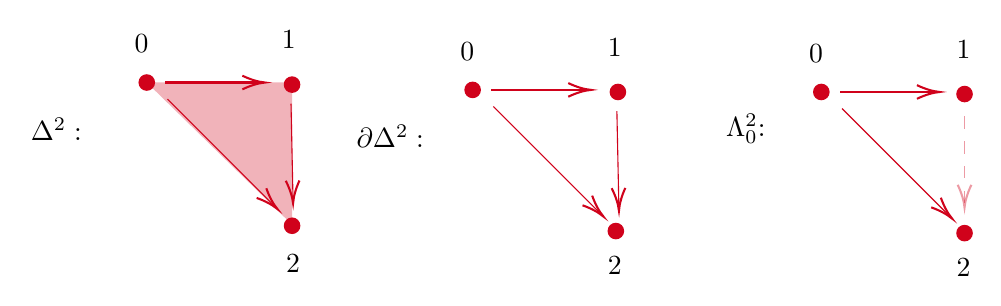
\begin{tikzpicture}[x=0.75pt,y=0.75pt,yscale=-1,xscale=1]
%uncomment if require: \path (0,240); %set diagram left start at 0, and has height of 240
%Shape: Free Drawing [id:dp20250857537916134] 
\draw  [color={rgb, 255:red, 208; green, 2; blue, 27 }  ,draw opacity=1 ][line width=6] [line join = round][line cap = round] (186.11,144.56) .. controls (186.11,144.56) and (186.11,144.56) .. (186.11,144.56) ;
%Shape: Free Drawing [id:dp8560192570653509] 
\draw  [color={rgb, 255:red, 208; green, 2; blue, 27 }  ,draw opacity=1 ][line width=6] [line join = round][line cap = round] (186.11,76.56) .. controls (186.11,76.56) and (186.11,76.56) .. (186.11,76.56) ;
%Shape: Free Drawing [id:dp26889850065743715] 
\draw  [color={rgb, 255:red, 208; green, 2; blue, 27 }  ,draw opacity=1 ][line width=6] [line join = round][line cap = round] (116.11,75.56) .. controls (116.11,75.56) and (116.11,75.56) .. (116.11,75.56) ;
%Straight Lines [id:da250770434621995] 
\draw [color={rgb, 255:red, 208; green, 2; blue, 27 }  ,draw opacity=1 ]   (185.61,85.78) -- (186.57,131.78) ;
\draw [shift={(186.61,133.78)}, rotate = 268.81] [color={rgb, 255:red, 208; green, 2; blue, 27 }  ,draw opacity=1 ][line width=0.75]    (10.93,-3.29) .. controls (6.95,-1.4) and (3.31,-0.3) .. (0,0) .. controls (3.31,0.3) and (6.95,1.4) .. (10.93,3.29)   ;
%Straight Lines [id:da5472503346326145] 
\draw [color={rgb, 255:red, 208; green, 2; blue, 27 }  ,draw opacity=1 ][line width=0.75]    (125.11,75.56) -- (171.11,75.56) ;
\draw [shift={(173.11,75.56)}, rotate = 180] [color={rgb, 255:red, 208; green, 2; blue, 27 }  ,draw opacity=1 ][line width=0.75]    (10.93,-3.29) .. controls (6.95,-1.4) and (3.31,-0.3) .. (0,0) .. controls (3.31,0.3) and (6.95,1.4) .. (10.93,3.29)   ;
%Straight Lines [id:da15503202104425817] 
\draw [color={rgb, 255:red, 208; green, 2; blue, 27 }  ,draw opacity=1 ]   (126.11,83.56) -- (177.7,135.14) ;
\draw [shift={(179.11,136.56)}, rotate = 225] [color={rgb, 255:red, 208; green, 2; blue, 27 }  ,draw opacity=1 ][line width=0.75]    (10.93,-3.29) .. controls (6.95,-1.4) and (3.31,-0.3) .. (0,0) .. controls (3.31,0.3) and (6.95,1.4) .. (10.93,3.29)   ;
%Shape: Polygon [id:ds5516763594874212] 
\draw  [draw opacity=0][fill={rgb, 255:red, 208; green, 2; blue, 27 }  ,fill opacity=0.3 ] (116.11,75.53) -- (186.11,75.53) -- (186.11,144.03) -- (116.11,75.53) -- cycle ;
%Shape: Free Drawing [id:dp6996632635597266] 
\draw  [color={rgb, 255:red, 208; green, 2; blue, 27 }  ,draw opacity=1 ][line width=6] [line join = round][line cap = round] (342.11,147.11) .. controls (342.11,147.11) and (342.11,147.11) .. (342.11,147.11) ;
%Shape: Free Drawing [id:dp23658558609305058] 
\draw  [color={rgb, 255:red, 208; green, 2; blue, 27 }  ,draw opacity=1 ][line width=6] [line join = round][line cap = round] (343.11,80.11) .. controls (343.11,80.11) and (343.11,80.11) .. (343.11,80.11) ;
%Shape: Free Drawing [id:dp5115039411399855] 
\draw  [color={rgb, 255:red, 208; green, 2; blue, 27 }  ,draw opacity=1 ][line width=6] [line join = round][line cap = round] (273.11,79.11) .. controls (273.11,79.11) and (273.11,79.11) .. (273.11,79.11) ;
%Straight Lines [id:da3744865515022133] 
\draw [color={rgb, 255:red, 208; green, 2; blue, 27 }  ,draw opacity=1 ]   (342.61,89.33) -- (343.57,135.33) ;
\draw [shift={(343.61,137.33)}, rotate = 268.81] [color={rgb, 255:red, 208; green, 2; blue, 27 }  ,draw opacity=1 ][line width=0.75]    (10.93,-3.29) .. controls (6.95,-1.4) and (3.31,-0.3) .. (0,0) .. controls (3.31,0.3) and (6.95,1.4) .. (10.93,3.29)   ;
%Straight Lines [id:da5413612535803476] 
\draw [color={rgb, 255:red, 208; green, 2; blue, 27 }  ,draw opacity=1 ][line width=0.75]    (282.11,79.11) -- (328.11,79.11) ;
\draw [shift={(330.11,79.11)}, rotate = 180] [color={rgb, 255:red, 208; green, 2; blue, 27 }  ,draw opacity=1 ][line width=0.75]    (10.93,-3.29) .. controls (6.95,-1.4) and (3.31,-0.3) .. (0,0) .. controls (3.31,0.3) and (6.95,1.4) .. (10.93,3.29)   ;
%Straight Lines [id:da17007192259087267] 
\draw [color={rgb, 255:red, 208; green, 2; blue, 27 }  ,draw opacity=1 ]   (283.11,87.11) -- (334.7,138.7) ;
\draw [shift={(336.11,140.11)}, rotate = 225] [color={rgb, 255:red, 208; green, 2; blue, 27 }  ,draw opacity=1 ][line width=0.75]    (10.93,-3.29) .. controls (6.95,-1.4) and (3.31,-0.3) .. (0,0) .. controls (3.31,0.3) and (6.95,1.4) .. (10.93,3.29)   ;
%Shape: Free Drawing [id:dp735452156887185] 
\draw  [color={rgb, 255:red, 208; green, 2; blue, 27 }  ,draw opacity=1 ][line width=6] [line join = round][line cap = round] (510.11,148.11) .. controls (510.11,148.11) and (510.11,148.11) .. (510.11,148.11) ;
%Shape: Free Drawing [id:dp12785217588086462] 
\draw  [color={rgb, 255:red, 208; green, 2; blue, 27 }  ,draw opacity=1 ][line width=6] [line join = round][line cap = round] (510.11,81.11) .. controls (510.11,81.11) and (510.11,81.11) .. (510.11,81.11) ;
%Shape: Free Drawing [id:dp4480432189571355] 
\draw  [color={rgb, 255:red, 208; green, 2; blue, 27 }  ,draw opacity=1 ][line width=6] [line join = round][line cap = round] (441.11,80.11) .. controls (441.11,80.11) and (441.11,80.11) .. (441.11,80.11) ;
%Straight Lines [id:da8320855200603781] 
\draw [color={rgb, 255:red, 208; green, 2; blue, 27 }  ,draw opacity=1 ][line width=0.75]    (450.11,80.11) -- (496.11,80.11) ;
\draw [shift={(498.11,80.11)}, rotate = 180] [color={rgb, 255:red, 208; green, 2; blue, 27 }  ,draw opacity=1 ][line width=0.75]    (10.93,-3.29) .. controls (6.95,-1.4) and (3.31,-0.3) .. (0,0) .. controls (3.31,0.3) and (6.95,1.4) .. (10.93,3.29)   ;
%Straight Lines [id:da24624276797536426] 
\draw [color={rgb, 255:red, 208; green, 2; blue, 27 }  ,draw opacity=1 ]   (451.11,88.11) -- (502.7,139.7) ;
\draw [shift={(504.11,141.11)}, rotate = 225] [color={rgb, 255:red, 208; green, 2; blue, 27 }  ,draw opacity=1 ][line width=0.75]    (10.93,-3.29) .. controls (6.95,-1.4) and (3.31,-0.3) .. (0,0) .. controls (3.31,0.3) and (6.95,1.4) .. (10.93,3.29)   ;
%Straight Lines [id:da36924497043702464] 
\draw [color={rgb, 255:red, 208; green, 2; blue, 27 }  ,draw opacity=0.4 ] [dash pattern={on 4.5pt off 4.5pt}]  (510.11,91.78) -- (510.11,133.78) ;
\draw [shift={(510.11,135.78)}, rotate = 270] [color={rgb, 255:red, 208; green, 2; blue, 27 }  ,draw opacity=0.4 ][line width=0.75]    (10.93,-3.29) .. controls (6.95,-1.4) and (3.31,-0.3) .. (0,0) .. controls (3.31,0.3) and (6.95,1.4) .. (10.93,3.29)   ;
% Text Node
\draw (59,91.4) node [anchor=north west][inner sep=0.75pt]    {$\Delta ^{2} :$};
% Text Node
\draw (109,51.4) node [anchor=north west][inner sep=0.75pt]    {$0$};
% Text Node
\draw (180,49.4) node [anchor=north west][inner sep=0.75pt]    {$1$};
% Text Node
\draw (182,157.4) node [anchor=north west][inner sep=0.75pt]    {$2$};
% Text Node
\draw (216,94.96) node [anchor=north west][inner sep=0.75pt]    {$\partial \Delta ^{2} :$};
% Text Node
\draw (266,54.96) node [anchor=north west][inner sep=0.75pt]    {$0$};
% Text Node
\draw (337,52.96) node [anchor=north west][inner sep=0.75pt]    {$1$};
% Text Node
\draw (337,157.96) node [anchor=north west][inner sep=0.75pt]    {$2$};
% Text Node
\draw (394,89.4) node [anchor=north west][inner sep=0.75pt]    {$\Lambda _{0}^{2}$:};
% Text Node
\draw (434,55.96) node [anchor=north west][inner sep=0.75pt]    {$0$};
% Text Node
\draw (505,53.96) node [anchor=north west][inner sep=0.75pt]    {$1$};
% Text Node
\draw (505,158.96) node [anchor=north west][inner sep=0.75pt]    {$2$};
\end{tikzpicture}\]
这解释了为什么说$\partial \Delta^n \simeq \bbS^{n-1}$.
此外,可以发现
\begin{proposition}\label{Pro:边界与尖角图表}
    单纯集范畴$\cate{sSet}$中有以下图表,上下两半分别交换($0\leq i < j \leq n$)
    \[\begin{tikzcd}
	{\Delta^{n-2}} & {\Delta^{n-1}} \\
	{\bigsqcup_{0\leq i' < j' \leq n}\Delta^{n-2}} & {\bigsqcup_{i'=0}^n\Delta^{n-1}} & {\partial\Delta^n} \\
	{\Delta^{n-2}} & {\Delta^{n-1}}
	\arrow["{\delta^{j-1}}", from=1-1, to=1-2]
	\arrow["{\iota_{i<j}}"', from=1-1, to=2-1]
	\arrow["{\iota_i}", from=1-2, to=2-2]
	\arrow["{\delta^i}", from=1-2, to=2-3]
	\arrow[shift left, from=2-1, to=2-2]
	\arrow[shift right, from=2-1, to=2-2]
	\arrow[from=2-2, to=2-3]
	\arrow["{\iota_{i<j}}", from=3-1, to=2-1]
	\arrow["{\delta^i}"', from=3-1, to=3-2]
	\arrow["{\iota_j}"', from=3-2, to=2-2]
	\arrow["{\delta^j}"', from=3-2, to=2-3]
    \end{tikzcd}\]
    其中$\bigsqcup$在$\cate{sSet}$中逐项选取,而$\iota_{i<j}$(或$\iota_i$)意谓向第$i<j$(或第$i$)项的嵌入;则有图表交换且中间部分为余等子.\\
    类似地,对$0\leq k \leq n$也有
    \[\begin{tikzcd}
	{\Delta^{n-2}} & {\Delta^{n-1}} \\
	{\bigsqcup_{0\leq i' < j' \leq n,i',j'\neq k}\Delta^{n-2}} & {\bigsqcup_{0\leq i'\leq n,i'\neq k}\Delta^{n-1}} & {\Lambda_k^n} \\
	{\Delta^{n-2}} & {\Delta^{n-1}}
	\arrow["{\delta^{j-1}}", from=1-1, to=1-2]
	\arrow["{\iota_{i<j}}"', from=1-1, to=2-1]
	\arrow["{\iota_i}", from=1-2, to=2-2]
	\arrow["{\delta^i}", from=1-2, to=2-3]
	\arrow[shift left, from=2-1, to=2-2]
	\arrow[shift right, from=2-1, to=2-2]
	\arrow[from=2-2, to=2-3]
	\arrow["{\iota_{i<j}}", from=3-1, to=2-1]
	\arrow["{\delta^i}"', from=3-1, to=3-2]
	\arrow["{\iota_j}"', from=3-2, to=2-2]
	\arrow["{\delta^j}"', from=3-2, to=2-3]
    \end{tikzcd}\]
    中间项也为余等子.
\end{proposition}
\begin{proof}
    验证即可.
\end{proof}
我们也可以将其视为$\partial \Delta^n$和$\Lambda_k^n$在``流水线''上的拼装过程,当然我们可以将其等价地表述为:
\begin{corollary}\label{推论:尖角变体}
    令$0 \leq i \leq n$为整数且$n >0$对于任意单纯集$S$,态射
    \begin{align*}
        \Hom_{\cate{sSet}}(\Lambda_k^n , S) &\to (S_{n-1})^n\\
        f &\mapsto \{f\circ \delta_n^j\}_{0\leq j \leq n,j \neq i}
    \end{align*}
    为单射,其像为``不完全''序列
    \[
        (\sigma_0,\cdots,\sigma_{i-1},\bullet,\sigma_{i+1},\cdots,\sigma_n)
    \]
    对于$k\in [n] \setminus \{i\}$且$j <k$的$k$ ,它满足等式$d_{n-1}^j(\sigma_k) = d_{n-1}^{k-1}(\sigma_j)$.
\end{corollary}
接下来引入脊(spine)的概念,它的意义将在后文得到阐述.
\begin{definition}[脊]
    对于$n$-单形$\Delta^n$定义子函子$I^n$为
    \[
    I^n := \{f\in \Hom([m],[n]): \Image(f) = \{j\} \text{或} \{j,j+1\}\}
    \]
\end{definition}
当$n=3$时$I^3 \subset \Delta^3$如下图所示,其中绿色虚线以及顶点为脊.
\[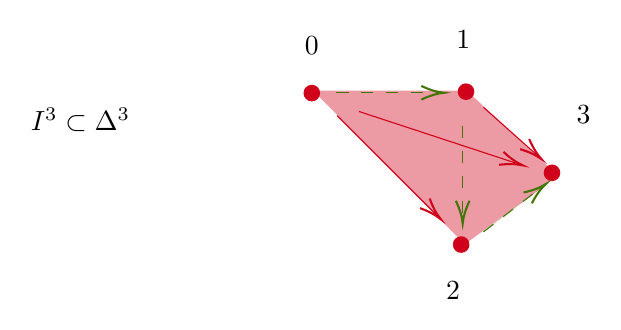
\begin{tikzpicture}[x=0.75pt,y=0.75pt,yscale=-1,xscale=1]
%uncomment if require: \path (0,184); %set diagram left start at 0, and has height of 184
%Straight Lines [id:da5832294719294788] 
\draw [draw opacity=0][fill={rgb, 255:red, 208; green, 2; blue, 27 }  ,fill opacity=0.4 ]   (317.33,62.5) -- (391.33,62.5) -- (435.33,103.5) -- (390.33,136.5) -- cycle ;
%Shape: Free Drawing [id:dp830584580009414] 
\draw  [color={rgb, 255:red, 208; green, 2; blue, 27 }  ,draw opacity=1 ][line width=6] [line join = round][line cap = round] (388.58,136.63) .. controls (388.58,136.63) and (388.58,136.63) .. (388.58,136.63) ;
%Shape: Free Drawing [id:dp3250839402586416] 
\draw  [color={rgb, 255:red, 208; green, 2; blue, 27 }  ,draw opacity=1 ][line width=6] [line join = round][line cap = round] (390.92,62.97) .. controls (390.92,62.97) and (390.92,62.97) .. (390.92,62.97) ;
%Shape: Free Drawing [id:dp7792822085041697] 
\draw  [color={rgb, 255:red, 208; green, 2; blue, 27 }  ,draw opacity=1 ][line width=6] [line join = round][line cap = round] (316.62,63.65) .. controls (316.62,63.65) and (316.62,63.65) .. (316.62,63.65) ;
%Shape: Free Drawing [id:dp19290457052024812] 
\draw  [color={rgb, 255:red, 208; green, 2; blue, 27 }  ,draw opacity=1 ][line width=6] [line join = round][line cap = round] (432.34,102.07) .. controls (432.34,102.07) and (432.34,102.07) .. (432.34,102.07) ;
%Straight Lines [id:da8563690958739549] 
\draw [color={rgb, 255:red, 65; green, 117; blue, 5 }  ,draw opacity=1 ] [dash pattern={on 4.5pt off 4.5pt}]  (328.33,63.5) -- (378.33,63.5) ;
\draw [shift={(380.33,63.5)}, rotate = 180] [color={rgb, 255:red, 65; green, 117; blue, 5 }  ,draw opacity=1 ][line width=0.75]    (10.93,-3.29) .. controls (6.95,-1.4) and (3.31,-0.3) .. (0,0) .. controls (3.31,0.3) and (6.95,1.4) .. (10.93,3.29)   ;
%Straight Lines [id:da6779286954756674] 
\draw [color={rgb, 255:red, 65; green, 117; blue, 5 }  ,draw opacity=1 ] [dash pattern={on 4.5pt off 4.5pt}]  (389.33,79.5) -- (389.33,124.5) ;
\draw [shift={(389.33,126.5)}, rotate = 270] [color={rgb, 255:red, 65; green, 117; blue, 5 }  ,draw opacity=1 ][line width=0.75]    (10.93,-3.29) .. controls (6.95,-1.4) and (3.31,-0.3) .. (0,0) .. controls (3.31,0.3) and (6.95,1.4) .. (10.93,3.29)   ;
%Straight Lines [id:da11968731710575464] 
\draw [color={rgb, 255:red, 65; green, 117; blue, 5 }  ,draw opacity=1 ][fill={rgb, 255:red, 65; green, 117; blue, 5 }  ,fill opacity=1 ] [dash pattern={on 4.5pt off 4.5pt}]  (399.33,130.5) -- (427.75,108.72) ;
\draw [shift={(429.33,107.5)}, rotate = 142.52] [color={rgb, 255:red, 65; green, 117; blue, 5 }  ,draw opacity=1 ][line width=0.75]    (10.93,-3.29) .. controls (6.95,-1.4) and (3.31,-0.3) .. (0,0) .. controls (3.31,0.3) and (6.95,1.4) .. (10.93,3.29)   ;
%Straight Lines [id:da17854575492651437] 
\draw [color={rgb, 255:red, 208; green, 2; blue, 27 }  ,draw opacity=1 ]   (328.83,74.5) -- (377.42,123.09) ;
\draw [shift={(378.83,124.5)}, rotate = 225] [color={rgb, 255:red, 208; green, 2; blue, 27 }  ,draw opacity=1 ][line width=0.75]    (10.93,-3.29) .. controls (6.95,-1.4) and (3.31,-0.3) .. (0,0) .. controls (3.31,0.3) and (6.95,1.4) .. (10.93,3.29)   ;
%Straight Lines [id:da8010680531974725] 
\draw [color={rgb, 255:red, 208; green, 2; blue, 27 }  ,draw opacity=1 ]   (339.33,72.5) -- (416.43,97.87) ;
\draw [shift={(418.33,98.5)}, rotate = 198.22] [color={rgb, 255:red, 208; green, 2; blue, 27 }  ,draw opacity=1 ][line width=0.75]    (10.93,-3.29) .. controls (6.95,-1.4) and (3.31,-0.3) .. (0,0) .. controls (3.31,0.3) and (6.95,1.4) .. (10.93,3.29)   ;
%Straight Lines [id:da06053624340237218] 
\draw [color={rgb, 255:red, 208; green, 2; blue, 27 }  ,draw opacity=1 ]   (399.33,70.5) -- (425.84,94.17) ;
\draw [shift={(427.33,95.5)}, rotate = 221.76] [color={rgb, 255:red, 208; green, 2; blue, 27 }  ,draw opacity=1 ][line width=0.75]    (10.93,-3.29) .. controls (6.95,-1.4) and (3.31,-0.3) .. (0,0) .. controls (3.31,0.3) and (6.95,1.4) .. (10.93,3.29)   ;
% Text Nod
\draw (385,32.4) node [anchor=north west][inner sep=0.75pt]    {$1$};
% Text Node
\draw (312,35.4) node [anchor=north west][inner sep=0.75pt]    {$0$};
% Text Node
\draw (443,68.4) node [anchor=north west][inner sep=0.75pt]    {$3$};
% Text Node
\draw (380.02,153.17) node [anchor=north west][inner sep=0.75pt]    {$2$};
% Text Node
\draw (180,69.4) node [anchor=north west][inner sep=0.75pt]    {$I^{3} \subset \Delta ^{3}$};
\end{tikzpicture}\]
不难发现$I^0 = \Delta^0$, $I^1 = \Delta^1$,且$I^n \subset \Lambda_i^n \subset \partial \Delta^n \subset \Delta^n$($1\leq i\leq n-1$或$n >3$).以及以下堆叠结构
\[
I^n = I^{n-1} \dsqcup{\Delta^0}\Delta^1.
\]
\section{单纯集的乘积}
\subsection{闭幺半范畴与$\cate{CGWH}$}\label{闭幺半与CGWH}
\begin{wenxintishi}
    为后文更加便利的叙述无穷范畴,我们来进行一点点题外话的讨论,这也是\parencite[Remark 1.1.1.7]{HTT}的更加详细的解释,不感兴趣的读者可以跳过.
\end{wenxintishi}
首先介绍闭幺半范畴的概念,不难发现单形对象可以和幺半范畴相联系.
\begin{definition}\label{Def:单形对象与幺半范畴}
    任何函子$F : \mathcal{C} \to \mathcal{D}$都相应地诱导$\mathsf{s}\mathcal{C}\to \mathsf{s}\mathcal{D}$,映资料$(X_n,d_i,s_j)_{n,i,j}$为$(FX_n,Fd_i,Fs_j)_{n,i,j}$.此外,有自明的关系式$\mathsf{s}(\mathcal{C}_1\times\mathcal{C}_2)\simeq {\mathsf{s}\mathcal{C}_1}\times{\mathsf{s}\mathcal{C}_2}$.\\
    将上述观察施于幺半范畴$\mathcal{C}$和双函子$\otimes:\mathcal{C}\times\mathcal{C} \to \mathcal{C}$,则对任意$X,Y\in \Obj(\mathsf{s}\mathcal{C})$可定义$X\otimes Y \in \Obj(\mathsf{s}\mathcal{C})$,其$n$次项为$X_n\otimes Y_n$,其面态射与退化态射分别形如$d_i \otimes d_j$和$s_i \otimes s_j$.
\end{definition}
\begin{definition}[闭幺半范畴]
    设$\mathcal{C}$为幺半范畴.当以下条件成立时,称$\mathcal{C}$为右(或左)闭幺半范畴:对所有对象$Y$,函子$ - \otimes Y : \mathcal{C} \to \mathcal{C}$(或$Y\otimes - : \mathcal{C} \to \mathcal{C}$)带有指定的右伴随.兼具左闭和右闭的幺半范畴称为闭幺半范畴.
\end{definition}
\begin{remark}
    我们考虑的幺半范畴均为辫幺半范畴,因此无需区分左闭右闭,此时$- \otimes Y$的右伴随记为$\underline{\Hom}(Y,-)$.
\end{remark}
一般而言,对任意范畴$\mathcal{C}_1$和$\mathcal{C}_2$之间的两对伴随函子$(F,G)$和$(F',G')$,任何$\varphi :F \to F'$都自然诱导了$\psi : G' \to G$.相反也是如此.诱导态射由交换图表
\[\begin{tikzcd}
	{\Hom(F'X,Y)} & {\Hom(X,G'Y)} \\
	{\Hom(FX,Y)} & {\Hom(X,GY)}
	\arrow["\sim"', from=1-1, to=1-2]
	\arrow["{(\varphi_X)^*}", from=1-1, to=2-1]
	\arrow["{(\psi_Y)_*}"', from=1-2, to=2-2]
	\arrow["\sim", from=2-1, to=2-2]
\end{tikzcd}\]
刻画.\\

作为应用,闭幺半范畴中的任何态射$Y \to Y'$诱导$\underline{\Hom}(Y', -)\to \underline{\Hom}(Y, -)$,所以闭幺半范畴的性质相当于在说存在双函子$\underline{\Hom}(-,-):\mathcal{C}^{\opposite} \times \mathcal{C} \to \mathcal{C}$以及一族典范双射
\begin{equation}\label{公式:内 Hom}
\tag{内 Hom}
   \Hom(X\otimes Y,Z) \simeq \Hom\left(X,\underline{\Hom}(Y,Z)\right), 
\end{equation}

它对于三个变元皆有函子性.\\

双函子$\underline{\Hom}(-,-)$也称为闭幺半范畴$\mathcal{C}$的内Hom.定义导致以下结论:
\begin{itemize}
    \item $\Hom(X,Z) \simeq \Hom(X\otimes \one,Z) \simeq \Hom(X,\underline{\Hom}(\one,Z))$,再由米田引理可知$Z \simeq \underline{\Hom}(\one,Z)$.
    \item 伴随对的单位态射给出$\coev_{X,Y}:X\to  \underline{\Hom}(Y,X\otimes Y)$,余单位态射给出$\ev_{Y,X}:\underline{\Hom}(Y,X)\otimes Y \to X$.
    \item 从合成
    \[\underline{\Hom}(Y,Z)\otimes(\underline{\Hom}(X,Y)\otimes X) \xrightarrow{\identity\otimes\ev_{X,Y}}\underline{\Hom}(Y,Z)\otimes Y\xrightarrow{\ev_{Y,Z}}Z\]
    以及伴随性质和结合约束可得
    \[
    \underline{\Hom}(Y,Z)\otimes\underline{\Hom}(X,Y)\to \underline{\Hom}(X,Z).
    \]
    \item 取$\coev_{\one,X}$得$\one \to \underline{\Hom}(X,X)$.
\end{itemize}
不难得到
\begin{proposition}
    设$\mathcal{C}$是闭幺半范畴,则有一族典范双射
    \[
    \Hom(X,Y) \simeq \Hom(\one,\underline{\Hom}(X,Y)),\quad X,Y \in \Obj(\mathcal{C}).
    \]
\end{proposition}
这说明内Hom可以得到Hom.\\

此外,伴随也可以内化到$\mathcal{C}$.
\begin{proposition}
    设$\mathcal{C}$是闭幺半范畴,则有一族同构
    \[
    \underline{\Hom}(X\otimes Y,Z)\simeq \underline{\Hom}(X,\underline{\Hom}(Y,Z));
    \]
    更精确地说,这是从$\mathcal{C}^{\opposite}\times \mathcal{C}^{\opposite}\times \mathcal{C} \to \mathcal{C}$的函子间的同构.
\end{proposition}
\begin{proof}
    考虑$\Hom(T,\underline{\Hom}(X\otimes Y,Z))$利用结合约束以及伴随同构证明$\Hom(T,\underline{\Hom}(X\otimes Y,Z))\rightiso \Hom(T,\underline{\Hom}(X,\underline{\Hom}(Y,Z)))$结合Yoneda引理可知结果.
\end{proof}
引入闭幺半范畴是为了进一步约化到双函子$\otimes$为积$\times$的情况,在这一情况下,会增加一个有趣的观察.
\begin{definition}[Cartesius闭]
    设$\mathcal{C}$是具备有限积的范畴.如果$(\mathcal{C},\times)$为闭幺半范畴,则称$\mathcal{C}$为Cartesius闭的.
\end{definition}
\begin{example}
\begin{enumerate}
    \item 集合范畴$\Set$是Cartesius闭的:取$\underline{\Hom}(X,Y) = Y^X$即可.
    \item 取$\mathcal{C} = \cate{Top}$,它具有许多良好性质,并且对积$\times$构成对称幺半范畴,但是它不是 Cartesian 闭的.
    \item 考虑全体小范畴构成的范畴$\cate{Cat}$,其中积为$\cal{C}_1\times \cdots \cal{C}_n$,而空积为$\bold{1}$.范畴$\cate{Cat}$是 Cartesian 闭的,这来自于以下简单的论断:指定双函子$\cal{A} \times \cal{B} \to \cal{C}$相当于指定函子$\cal{A} \to \cal{C}^{\cal{B}}$也相当于指定函子$\cal{B} \to \cal{C}^{\cal{A}}$.
\end{enumerate}
\end{example}
由于映射空间在拓扑学中俯拾即是,为解决$\cate{Top}$不是 Cartesian 闭的问题,我们引入紧生成空间与紧生成弱 Hausdorff 空间.两者都是方便的空间范畴,在$\infty$-范畴理论中,使用紧生成弱 Hausdorff 空间更多一些.\\
首先,回顾一下紧生成空间的定义,根据Bourbaki的定义,紧空间意谓紧且Hausdorff的空间.
\begin{definition}[弱Hausdorff]\label{定义:弱Hausdorff}
    设$X$为拓扑空间, $K$为紧空间,若对于任意连续映射$f: K \to X$都有$f(K)$是$X$中的闭集,则称$X$是弱Hausdorff的.
\end{definition}
\begin{example}
    Hausdorff空间是弱 Hausdorff 的.
\end{example}
这种空间的分离性介于T$_1$与Hausdorff之间.
\begin{definition}[紧闭子空间]\label{定义:紧闭子空间}
    设$X$为拓扑空间, $A \subset X$为其子空间, $K$为紧空间,若对于任意映射$f : K \to X$都有$f^{-1}(A)$为$K$中的闭集,则称$A$是$X$的紧闭子空间.\footnote{注意,不一定在$X$上闭}
\end{definition}
\begin{definition}[Kelly空间]
    设$X$为拓扑空间,若其每个紧闭子空间在$X$上都是闭的,则称$X$为Kelly空间,简称$k$-空间.
\end{definition}
\begin{definition}[紧生成空间]\label{定义:紧生成空间}
    设$X$为拓扑空间,以$X$中的紧闭子集作为闭集构成一个新的拓扑空间$kX$,有恒等映射$kX \to X$.若$kX = X$,则称$X$是紧生成的.记$\cate{CG}$为$\cate{Top}$中所有紧生成空间构成的范畴,当然也可以说是$k$-空间构成的范畴.
\end{definition}
\begin{proposition}\label{命题:紧生成化与嵌入函子伴随}
    由$X \mapsto kX$给出的函子$k : \cate{Top} \to \cate{CG}$是嵌入函子$\iota: \cate{CG} \to \cate{Top}$的右伴随.
\end{proposition}
\begin{proof}
    记$X \in \cate{CG}$, $Y\in \cate{Top}$,欲证
    \[
    \Hom_{\cate{CG}}(X,kY)\simeq \Hom_{\cate{Top}}(\iota X,Y),
    \]
    只需证明$f : X \to Y$连续当且仅当$f : X \to kY$连续即可.
    \begin{enumerate}
        \item[($\Rightarrow$)]假设$f: X\to Y$连续,则令$Z \subset Y$为紧闭子集考虑$f^{-1}(Z)$.对任意紧空间$K$,映射$g: K \to X$,由于$f\circ g : K \to Y$,因此$(f\circ g)^{-1}(Z)$在$K$中是闭的,这意味着$f^{-1}(Z)$为$X$中的紧闭子集,而$X$为紧生成空间,即$f^{-1}(Z)$在$X$中闭,从而$kY$中的闭集在$f$的逆像为$X$中的闭集从而$f: X \to kY$连续.
        \item[($\Leftarrow$)]由于$kY \to Y$连续,因此考虑复合即可.
    \end{enumerate}
\end{proof}
\begin{proposition}\label{Pro:紧生成空间商映射}
    若$X \in \cate{CG}$, $\pr: X\to Y$为商映射,则$Y\in \cate{CG}$.
\end{proposition}
\begin{proof}
    由于商映射为使得$\pr : X \to Y$连续的最细的映射且有分解$\pr : X \to kY \to Y$,因此$Y = kY$.
\end{proof}
\begin{theorem}[$\cate{CG}$的完备性]
    范畴$\cate{CG}$完备且余完备.其余极限继承相应空间在$\cate{Top}$中的余极限,而极限由$k$作用于相应空间在$\cate{Top}$中的极限得到.
\end{theorem}
\begin{proof}
    设$\mathcal{I}$为指标范畴, $F \in \Fct(\mathcal{I},\cate{CG})$, $\hat{F} = \iota \circ F$.由于$\iota$为左伴随,保$\indlim$,因此只需要证明$\cate{CG}$中对象在$\cate{Top}$的余极限仍在$\cate{CG}$中即可,由于命题\ref{Pro:紧生成空间商映射},只需要证明$\bigsqcup_{i\in \mathcal{I}}F(i)$在$\cate{CG}$中即可,这是显然的.而后由于$k$为右伴随,因此保$\prolim$,即
    \[
    \underset{i\in \mathcal{I}}{\prolim} F(i) = \underset{i\in \mathcal{I}}{\prolim} (k\circ \hat{F}(i)) = k \underset{i\in \mathcal{I}}{\prolim} \hat{F}(i).
    \]
\end{proof}
\begin{corollary}
    令$\{X_i\}_{i\in I}$为$\cate{CG}$中的一族对象.则它们在$\cate{CG}$中的乘积为
    \[
     k(\prod_{i\in I}X_i)
    \]
    此处$\prod_{i\in I}X_i$为在拓扑空间中的乘积.
\end{corollary}
\begin{definition}[紧生成弱Hausdorff空间]\label{Def:紧生成弱Hausdorff空间}
    设$X$为拓扑空间,若其是弱Hausdorff的$k$-空间,则称其为紧生成空间,其构成的范畴记为$\cate{CGWH}$.
\end{definition}
\begin{example}
    引理\ref{Lem:单纯集几何实现与CW-复形}可知$|\cate{sSet}| \subset \cate{CGWH}$.
\end{example}
\begin{proposition}
    设$X$为弱Hausdorff空间, $K$为紧空间,若$f : K \to X$连续,则$f(K)$为紧空间.
\end{proposition}
\begin{proof}
    由于$K$紧且$X$弱Hausdorff,由定义即知$f(K)$闭,而由连续映射保持紧性知$f(K)$紧,此外得知$f$为闭映射.而后考虑$x_1,x_2 \in f(K)$由于$X$为弱Hausdorff空间, $\{x_1\}$和$\{x_2\}$为闭子集,因此考虑其逆像得知$f^{-1}(x_1)$与$f^{-1}(x_2)$无交,而$K$紧Hausdorff,从而存在$U_1,U_2$为$K$中开集使得$f^{-1}(x_1)\in U_1$而$f^{-1}(x_2)\in U_2$,即$x_2\in K-U_1$而$x_1 \in K-U_2$.考虑$f(K) - f(K-U_i)$($i=1,2$)便得到包含$x_1$和$x_2$的无交开集.
\end{proof}
\begin{proposition}
    设$X$为紧生成空间,则$X$弱Hausdorff当且仅当对角线子空间$\delta_X$在$X\times X$中闭,此处$X \times X$为$\cate{CG}$中的乘积.
\end{proposition}
\begin{proof}
    设$X \in  \cate{CGWH}$,现证$\delta_X$紧闭.考虑
    \[
    f=(f_1,f_2) : K \to X\times X, f_i : K \to X
    \]
    $K$为紧空间,记
    \[
    L = f_1(K) \cap f_2(K)
    \]
    可知$L$为紧空间.考虑对角线$\delta_L$,由于$L$为紧空间, $\delta_L$为$X\times X$的紧子空间,而$X$紧生成,因此$\delta_L$在$X\times X$中闭.即$f^{-1}(\delta_X) = f^{-1}(\delta_L)$闭.\\
    反过来只需证明若$K$为紧空间$f: K\to X$连续,则$f(K)$紧闭即可.不妨设$L$为紧空间, $g: L \to X$连续,考虑
    \[
    (f,g): K \times L \to X\times X.
    \]
    则
    \[
    g^{-1}(f(K)) = (f,g)^{-1}(\delta_X)
    \]
    为闭集,即$f(K)$紧闭.
\end{proof}
\begin{corollary}\label{Cor:CG乘积也在CGWH中}
    设$\{X_i\}$为$\cate{CGWH}$中的一族对象,则它们在$\cate{CG}$的乘积也在$\cate{CGWH}$中.
\end{corollary}
\begin{proposition}
    函子$h : \cate{CG} \to \cate{CGWH}$是嵌入$\iota': \cate{CGWH}\to \cate{CG}$的左伴随.
\end{proposition}
\begin{theorem}[$\cate{CGWH}$的完备性]\label{The:CGWH的完备性}
    范畴$\cate{CGWH}$完备且余完备.极限继承自$\cate{CG}$而余极限来自$h$作用于$\cate{CG}$.
\end{theorem}
\begin{proof}
    与$\cate{CG}$完备且余完备的证明是类似的.唯一不平凡的是需要使用推论\ref{Cor:CG乘积也在CGWH中}即可得知乘积存在,而后由范畴中构造极限的方式可以证明极限确实继承自$\cate{CG}$.
\end{proof}
\begin{proposition}
    $\cate{CGWH}$是 Cartesian 闭的.
\end{proposition}
\begin{proof}   
见\parencite[Proposition 2.12]{StricklandCGWH}
\end{proof}
在对于同伦论的研究中,使用紧生成弱Hausdorff空间范畴$\cate{CGWH}$是更加方便的.因为$\cate{Top}$不是Cartesius闭的\footnote{由于不保\href{https://ncatlab.org/nlab/show/regular+epimorphism}{正则满态射(regular epimorphism)}},而\begin{tikzcd}
	{\cate{CGWH}} & {\cate{Top}}
	\arrow["{\text{包含}}", shift left, from=1-1, to=1-2]
	\arrow["k", shift left, from=1-2, to=1-1]
    \end{tikzcd}
中$\cate{CGWH}$为Cartesius闭范畴;可以证明前文伴随对中包含函子保$\indlim$但不保积.由于前文中$n$-单纯集的几何实现$|\Delta^n|$是一个紧生成弱Hausdorff空间,并且,因此几何实现(或奇异集)中的粘合(或取$\Hom$)可在$\cate{CGWH}$中操作(因所论的极限都在$\cate{CGWH}$中存在)因此定理\ref{The:几何实现是奇异集函子的左伴随}中伴随对分为两段
\[\begin{tikzcd}
	{\cate{sSet}} & {\cate{CGWH}} & {\cate{Top}}
	\arrow["{|-|}", shift left, from=1-1, to=1-2]
	\arrow["\Sing", shift left, from=1-2, to=1-1]
	\arrow["{\text{包含}}", shift left, from=1-2, to=1-3]
	\arrow["k", shift left, from=1-3, to=1-2]
\end{tikzcd}\]
对任意两个单纯集$X$和$Y$,就可以定义它们的逐项积
\begin{align*}
    (X\times Y)_n &= X_n \times Y_n\\
    d_i(x,y) &= (d_i(x),d_i(y))\\
    s_j(x,y) &= (s_j(x),s_j(y)).
\end{align*}
这是定义\ref{Def:单形对象与幺半范畴}中取$(\cate{Set},\times)$的产物,以下结果表明其承载几何意义.
\begin{theorem}\label{The:单纯集的积的几何意义}
    对于单纯集$X$和$Y$,我们有$\cate{CGWH}$中的典范同构
    \[
    |X\times Y| \simeq |X|\times |Y|
    \]
    推而广之, $\cate{CGWH}$版本的$|-|$保有限$\prolim$.若$X$和$Y$其中之一仅有有限多个非退化单纯形,则$|X\times Y| \simeq |X|\times |Y|$在$\cate{Top}$中也成立.
\end{theorem}
\begin{proof}
    在\parencite[Chapter 3, $\S$3,(3.1)]{Gabriel-Zisman67}中已经证明几何实现与余极限以及有限极限可交换而后在\parencite[Chapter 3, $\S$3,(3.5)]{Gabriel-Zisman67}中说明对于任意单纯集$X,Y$都有
    \[
    |X \times Y| \rightiso k(|X| \times |Y|)
    \]
    因此在$\cate{CGWH}$中有典范同构
    \[
    |X \times Y| \rightiso |X| \times |Y|
    \]
\end{proof}
\begin{remark}
    事实上,我们有\href{https://ncatlab.org/nlab/show/convenient+category+of+topological+spaces}{方便的空间范畴(convenient category of topological spaces)}一说.
\end{remark}
\begin{corollary}
    记$\cate{Grp}$,若单纯形集$X$可以升级为$\cate{Grp}^{\Delta^{\opposite}}$的对象,则$|X|$也自然地具有拓扑群结构;对于其它代数结构也有类似的结果.
\end{corollary}
在单纯集中,结合定理\ref{The:单纯集的积的几何意义}可以很自然地定义出同伦来,对于$\cate{sSet}$中的态射$f,g : X \twoheadrightarrow Y$定义$g$到$f$的(单纯)同伦为态射$H: X\times \Delta^1 \to Y$,使得下图交换:
\[\begin{tikzcd}
	{X\times \Delta^0} && X \\
	{X\times \Delta^1} && Y \\
	{X\times \Delta^0} && X
	\arrow["\sim", from=1-1, to=1-3]
	\arrow["{\identity_X \times d_0}"', from=1-1, to=2-1]
	\arrow["f"{description}, from=1-3, to=2-3]
	\arrow["H"{description}, from=2-1, to=2-3]
	\arrow["{\identity_X\times d_1}", from=3-1, to=2-1]
	\arrow["\sim"', from=3-1, to=3-3]
	\arrow["g"{description}, from=3-3, to=2-3]
\end{tikzcd}\]
熟悉模型范畴的读者应当可以看出此处\href{https://ncatlab.org/nlab/show/homotopy+in+a+model+category}{同伦}为使用\href{https://ncatlab.org/nlab/show/cylinder+object}{柱对象}定义的左同伦,自然也有使用\href{https://ncatlab.org/nlab/show/path+space+object}{路径对象}\footnote{柱对象和路径对象分别模仿$X \times I\to Y$和$X \to Y^I$两种情况.}所定义出的右同伦(或称余单纯同伦)$F : X \to Y^{\Delta^1}$,使得下图交换:
\[\begin{tikzcd}
	Y && {Y^{\Delta^0}} \\
	X && {Y^{\Delta^1}} \\
	Y && {Y^{\Delta^0}}
	\arrow["\sim", from=1-3, to=1-1]
	\arrow["f"', from=2-1, to=1-1]
	\arrow["F"{description}, from=2-1, to=2-3]
	\arrow["g", from=2-1, to=3-1]
	\arrow["{(d_1)^*}", from=2-3, to=1-3]
	\arrow["{(d_0)^*}"', from=2-3, to=3-3]
	\arrow["\sim"', from=3-3, to=3-1]
\end{tikzcd}\]

可以证明在拟范畴中这两种同伦是一致的,具有关心左右同伦及其一致性雅兴的读者,敬请阅读\parencite[11.4 and 11.7]{RezkQuasi-Cat}.\\
最后,我们探讨$\cate{sSet}$的 Cartesian 闭性.
\begin{definition}
    对于 $X,Y\in \Obj(\cate{sSet})$, 定义$\Fct(X,Y) = \iHom_{\cate{sSet}}(X,Y)\in \Obj(\cate{sSet})$如下
    \[
    \Fct(X,Y)_n := \Hom_{\cate{sSet}}(X\times \Delta^n,Y),\quad n\in \Z_{\geq 0},
    \]
    而对$\Delta$的任意态射$f: [m]\to [n]$,定义$f^* : \Fct(X,Y)_m \to \Fct(X,Y)_n$为沿
    \[
    \identity \times f : X \times \Delta^m \to X \times \Delta^n
    \]
    的拉回.另外,求值态射
    \[
    \ev_{X,Y}: \Fct(X,Y)\times X \to Y
    \]
    定义如下:$(\varphi,x)\in \Hom_{\cate{sSet}}(X\times \Delta^n,Y)_n\times X_n$的像为$\ev_{X,Y,n}(\varphi,x) := \varphi(x,\identity_{[n]})\in Y_n$(回忆到$(\Delta^n)_n = \Hom([n],[n]) = \End([n])$).
\end{definition}
必须验证$\ev_{X,Y}$确实是$\cate{sSet}$的态射.这毫不困难:给定$f: [m] \to [n]$和$(\varphi,x)\in \Fct(X,Y)_n \times X_n$,有
\begin{align*}
    \ev_{X,Y,m}(f^*(\varphi),f^*(x)) &= \left((\identity_X\times f)^*\varphi\right) \left(f^*(x),\identity_{[m]}\right)\\
    &= \varphi\left(\underset{\in X_m \times(\Delta^n)_m}{\underbrace{f^*(x),f}}\right) = \varphi\left(f^*(x),f^*\identity_{[n]}\right)\\
    &= f^*\left(\varphi(x,\identity_{[n]})\right) = f^*\left(\ev_{X,Y,n}(\varphi,x)\right).
\end{align*}
变动$X,Y$,给出函子$\Fct : \cate{sSet}^{\opposite}\times \cate{sSet} \to \cate{sSet}$而$\ev$对$X$和$Y$是典范的.
\begin{theorem}[$\cate{sSet}$是 Cartesian 闭的]\label{定理:sSet是Cartesian闭的}
    对所有$X,Y,Z\in \Obj(\cate{sSet})$,有典范双射
    \[
    \Hom_{\cate{sSet}}(X,\Fct(Y,Z))\xleftrightarrow{1:1} \Hom_{\cate{sSet}}(X\times Y,Z)
    \]
    它映$g:X \to \Fct(Y,Z)$为以下态射的合成
    \[
    X\times Y \xrightarrow{g\times \identity_{Y}}\Fct(Y,Z) \times Y \xrightarrow{\ev_{Y,Z}}Z.
    \]
    它映$h : X \times Y \to Z$为以下态射:设$n\in \Z_{\geq 0}$而$x\in X_n$,对应于态射$\iota_x : \Delta^n \to X$,则$x$的像是以下合成
    \[
    Y\times \Delta^n \xrightarrow{\identity_Y \times \iota_x}Y \times X\xrightarrow[\sim]{\text{换位}} X \times Y \xrightarrow{h} Z
    \]
    结合公式(\ref{公式:内 Hom})可判断$\cate{sSet}$是Cartesian闭的.
\end{theorem}
\begin{proof}
    验证即可.
\end{proof}
\subsection{标准单形的乘积}
接下来我们讨论$X = \Delta^p$和$Y = \Delta^q$时所对应的$\Delta^p \times \Delta^q$,比方说,如何分类$\Delta^p \times \Delta^q$上的非退化单形?问题的答案非但有助于理解积的几何实现,相关构造也是之后需要的.\\
首先,任两个偏序集$S_1$和$S_2$的积$S_1 \times S_2$通过$(a_1,a_2) \leq (b_1,b_2) \Leftrightarrow a_1 \leq b_1,a_2 \leq b_2$成为偏序集,这也相当于取它们对应范畴的积.
\begin{definition}
    设$p,q\in \Z_{\geq 0}$.所谓$(p,q)$-重组,意谓保序单射$\sigma : [p+q]\to [p]\times [q]$.
\end{definition}
对任意$n\in \Z_{\geq 0}$,指定保序映射$[n] \to [p]\times [q]$相当于指定一对保序映射$\sigma_{-} : [n] \to [p]$以及$\sigma_{+}:[n] \to [q]$;也相当于指定$\Delta^p \times \Delta^q$的一个$n$-单形.要求$i \mapsto (\sigma_{-}(i),\sigma_{+}(i))$的轨迹不停顿($i = 0,\cdots,n$).对于$n = p+q$时可以图解为
\[\begin{tikzpicture}[x=0.75pt,y=0.75pt,yscale=-1,xscale=1]
%uncomment if require: \path (0,300); %set diagram left start at 0, and has height of 300

%Shape: Square [id:dp9200085151915061] 
\draw  [color={rgb, 255:red, 155; green, 155; blue, 155 }  ,draw opacity=1 ] (127,81) -- (161.11,81) -- (161.11,115.11) -- (127,115.11) -- cycle ;
%Shape: Square [id:dp7316878376868328] 
\draw  [color={rgb, 255:red, 155; green, 155; blue, 155 }  ,draw opacity=1 ] (161.11,81) -- (195.22,81) -- (195.22,115.11) -- (161.11,115.11) -- cycle ;
%Shape: Square [id:dp7345201478772678] 
\draw  [color={rgb, 255:red, 155; green, 155; blue, 155 }  ,draw opacity=1 ] (127,115.11) -- (161.11,115.11) -- (161.11,149.22) -- (127,149.22) -- cycle ;
%Shape: Square [id:dp9194245889335557] 
\draw  [color={rgb, 255:red, 155; green, 155; blue, 155 }  ,draw opacity=1 ] (161.11,115.11) -- (195.22,115.11) -- (195.22,149.22) -- (161.11,149.22) -- cycle ;
%Shape: Square [id:dp9819463147507028] 
\draw  [color={rgb, 255:red, 155; green, 155; blue, 155 }  ,draw opacity=1 ] (195.22,81) -- (229.33,81) -- (229.33,115.11) -- (195.22,115.11) -- cycle ;
%Shape: Square [id:dp2144558429344554] 
\draw  [color={rgb, 255:red, 155; green, 155; blue, 155 }  ,draw opacity=1 ] (229.33,81) -- (263.44,81) -- (263.44,115.11) -- (229.33,115.11) -- cycle ;
%Shape: Square [id:dp03657410340992695] 
\draw  [color={rgb, 255:red, 155; green, 155; blue, 155 }  ,draw opacity=1 ] (263.44,81) -- (297.56,81) -- (297.56,115.11) -- (263.44,115.11) -- cycle ;
%Shape: Square [id:dp12006168557256958] 
\draw  [color={rgb, 255:red, 155; green, 155; blue, 155 }  ,draw opacity=1 ] (195.22,115.11) -- (229.33,115.11) -- (229.33,149.22) -- (195.22,149.22) -- cycle ;
%Shape: Square [id:dp1242866028192735] 
\draw  [color={rgb, 255:red, 155; green, 155; blue, 155 }  ,draw opacity=1 ] (229.33,115.11) -- (263.44,115.11) -- (263.44,149.22) -- (229.33,149.22) -- cycle ;
%Shape: Square [id:dp648778429497445] 
\draw  [color={rgb, 255:red, 155; green, 155; blue, 155 }  ,draw opacity=1 ] (263.44,115.11) -- (297.56,115.11) -- (297.56,149.22) -- (263.44,149.22) -- cycle ;
%Shape: Square [id:dp2740991741808232] 
\draw  [color={rgb, 255:red, 155; green, 155; blue, 155 }  ,draw opacity=1 ] (127,149.22) -- (161.11,149.22) -- (161.11,183.33) -- (127,183.33) -- cycle ;
%Shape: Square [id:dp37269635233617526] 
\draw  [color={rgb, 255:red, 155; green, 155; blue, 155 }  ,draw opacity=1 ] (161.11,149.22) -- (195.22,149.22) -- (195.22,183.33) -- (161.11,183.33) -- cycle ;
%Shape: Square [id:dp9507679799360924] 
\draw  [color={rgb, 255:red, 155; green, 155; blue, 155 }  ,draw opacity=1 ] (195.22,149.22) -- (229.33,149.22) -- (229.33,183.33) -- (195.22,183.33) -- cycle ;
%Shape: Square [id:dp5843515974208688] 
\draw  [color={rgb, 255:red, 155; green, 155; blue, 155 }  ,draw opacity=1 ] (229.33,149.22) -- (263.44,149.22) -- (263.44,183.33) -- (229.33,183.33) -- cycle ;
%Shape: Square [id:dp9355071433648059] 
\draw  [color={rgb, 255:red, 155; green, 155; blue, 155 }  ,draw opacity=1 ] (263.44,149.22) -- (297.56,149.22) -- (297.56,183.33) -- (263.44,183.33) -- cycle ;
%Shape: Square [id:dp8376323002057664] 
\draw  [color={rgb, 255:red, 155; green, 155; blue, 155 }  ,draw opacity=1 ] (127,183.33) -- (161.11,183.33) -- (161.11,217.44) -- (127,217.44) -- cycle ;
%Shape: Square [id:dp4248702782223266] 
\draw  [color={rgb, 255:red, 155; green, 155; blue, 155 }  ,draw opacity=1 ] (161.11,183.33) -- (195.22,183.33) -- (195.22,217.44) -- (161.11,217.44) -- cycle ;
%Shape: Square [id:dp9607310045186002] 
\draw  [color={rgb, 255:red, 155; green, 155; blue, 155 }  ,draw opacity=1 ] (195.22,183.33) -- (229.33,183.33) -- (229.33,217.44) -- (195.22,217.44) -- cycle ;
%Shape: Square [id:dp25732339354119693] 
\draw  [color={rgb, 255:red, 155; green, 155; blue, 155 }  ,draw opacity=1 ] (229.33,183.33) -- (263.44,183.33) -- (263.44,217.44) -- (229.33,217.44) -- cycle ;
%Shape: Square [id:dp23379818350891357] 
\draw  [color={rgb, 255:red, 155; green, 155; blue, 155 }  ,draw opacity=1 ] (263.44,183.33) -- (297.56,183.33) -- (297.56,217.44) -- (263.44,217.44) -- cycle ;
%Straight Lines [id:da7298797239711685] 
\draw [line width=1.5]    (127,217.44) -- (161.11,217.44) -- (161.11,183.33) -- (195.22,183.33) -- (229.33,183.33) -- (229.33,149.22) -- (263.44,149.22) -- (263.44,81) -- (297.56,81) ;

% Text Node
\draw (75,216.4) node [anchor=north west][inner sep=0.75pt]    {$i=0$};
% Text Node
\draw (309,61.4) node [anchor=north west][inner sep=0.75pt]    {$( p,q)$};
% Text Node
\draw (380,137) node [anchor=north west][inner sep=0.75pt]   [align=left] {恰好移动 $\displaystyle p+q$ 步};
\end{tikzpicture}\]
于是对于$(p,q)$-重组$\sigma$可以定义
\begin{align*}
    I_{\pm} &:= \{1\leq i \leq p+q : \sigma_{\pm}(i-1) < \sigma_{\pm}(i)\}\\
    &=\{1\leq i \leq p+q:\sigma_{\pm}(i-1) = \sigma_{\pm}(i)-1\}\\
    &=\{1\leq i \leq p+q:\sigma_{\mp}(i-1) = \sigma_{\mp}(i)\},
\end{align*}
它们满足$I_+ \sqcup I_- = \{1,\cdots,p+q\}$.子集$I_+$(或$I_-$)如上图的向上(或向右)部分,故$(p,q)$-重组的另一种观点是视其为$p$个$\to$以及$q$个$\uparrow$的排列,不难发现有${p+q}\choose{p}$种.这些观察顺带说明$\sigma_{+}$和$\sigma_{-}$对于$(p,q)$-重组是保序满射.
\begin{proposition}
    设$p,q\in \Z_{\geq 0}$.考虑$\Delta^p \times \Delta^q$的$n$-单形,亦即保序映射$\sigma : [n] \to [p]\times [q]$.命$(p_i,q_i):=\sigma(i)$, $(p',q'):= (p_n-p_0,q_n-q_0)$,则$\sigma$非退化当且仅当下述条件成立
    \begin{enumerate}
        \item $p'+q' = n$;
        \item $\sigma$分解为$(p',q')$-重组$\sigma' : [n] \to [p']+[q']$和形如$f\times g$的保序单射$[p']\times [q'] \hookrightarrow [p]\times [q]$.
    \end{enumerate}
\end{proposition}
\begin{proof}
    让$\sigma$对应到保序映射对$(\sigma_-,\sigma_+)$.不难发现$\sigma$非退化相当于说$i\mapsto (p_i,q_i)$的轨迹不停顿.因此命题是自明的.
\end{proof}
基于非退化单纯形的描述,读者不妨发挥想象力揣摩$|\Delta^p \times \Delta^q| \simeq |\Delta^p| \times |\Delta^q|$在$(p,q) =(1,1)$和$(2,1)$时的道理.例如下图是将$|\Delta^2 |\times |\Delta^1|$剖分为$3$个四面体的结果,对应于$3 = {3\choose 2}$个$(2,1)$-重组.
\[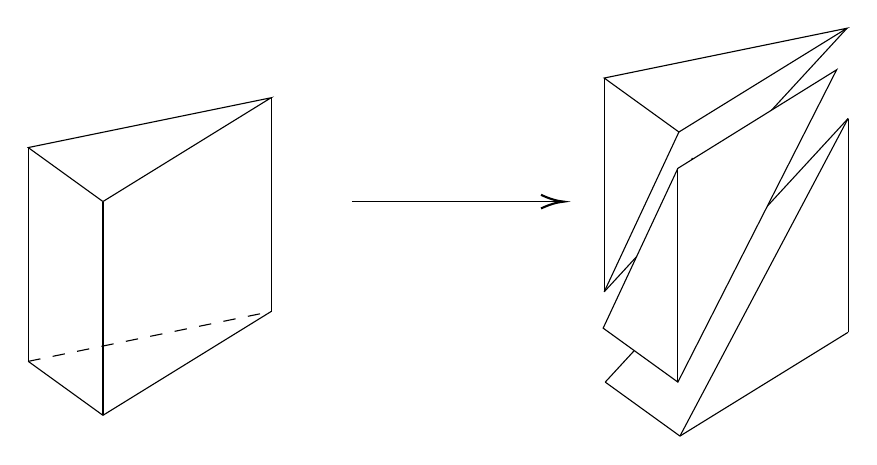
\begin{tikzpicture}[x=0.75pt,y=0.75pt,yscale=-1,xscale=1]
%uncomment if require: \path (0,300); %set diagram left start at 0, and has height of 300

%Straight Lines [id:da7320988534337254] 
\draw    (206.11,89.95) -- (89.11,113.95) -- (125.11,139.95) -- cycle ;
%Straight Lines [id:da7731734512646173] 
\draw    (89.11,113.95) -- (89.11,216.95) ;
%Straight Lines [id:da8693410695407291] 
\draw    (125.11,139.95) -- (125.11,242.95) ;
%Straight Lines [id:da34778996424608755] 
\draw    (206.11,89.95) -- (206.11,192.95) ;
%Straight Lines [id:da6485703140189338] 
\draw    (89.11,216.95) -- (125.11,242.95) -- (206.11,192.95) ;
%Straight Lines [id:da4428671688368293] 
\draw  [dash pattern={on 4.5pt off 4.5pt}]  (89.11,216.95) -- (206.11,192.95) ;
%Straight Lines [id:da6469878563000044] 
\draw    (245,140) -- (345.11,140) ;
\draw [shift={(347.11,140)}, rotate = 180] [color={rgb, 255:red, 0; green, 0; blue, 0 }  ][line width=0.75]    (10.93,-3.29) .. controls (6.95,-1.4) and (3.31,-0.3) .. (0,0) .. controls (3.31,0.3) and (6.95,1.4) .. (10.93,3.29)   ;
%Straight Lines [id:da9786602942081664] 
\draw    (366.61,80.45) -- (366.61,183.45) ;
%Straight Lines [id:da09611235081394187] 
\draw    (373.11,195.95) -- (409.11,118.95) ;
%Straight Lines [id:da03367413546565712] 
\draw    (402.61,106.45) -- (366.61,183.45) ;
%Straight Lines [id:da5015870642967339] 
\draw    (366.61,183.45) -- (483.61,56.45) ;
%Straight Lines [id:da8842588269678069] 
\draw    (483.61,56.45) -- (366.61,80.45) -- (402.61,106.45) -- cycle ;
%Straight Lines [id:da2697482316833171] 
\draw    (367.11,226.95) -- (403.11,252.95) -- (484.11,202.95) ;
%Straight Lines [id:da33617365628102003] 
\draw    (484.11,99.95) -- (484.11,202.95) ;
%Straight Lines [id:da782615014690863] 
\draw    (403.11,252.95) -- (484.11,99.95) ;
%Straight Lines [id:da3404844465403125] 
\draw    (367.11,226.95) -- (484.11,99.95) ;
%Shape: Polygon [id:ds9600948394944278] 
\draw  [fill={rgb, 255:red, 255; green, 255; blue, 255 }  ,fill opacity=1 ] (478.61,76.45) -- (402.11,226.95) -- (402.11,226.95) -- (366.11,200.95) -- (402.11,123.95) -- cycle ;
%Straight Lines [id:da037161638623682824] 
\draw    (402.11,123.95) -- (402.11,159.95) -- (402.11,226.95) ;
\end{tikzpicture}
\]
\begin{definition}
    设$\sigma$为$(p,q)$-重组,其符号定义为
    \[
    \sgn(\sigma) := (-1)^{|I_{\sigma}|}, I_{\sigma}:= \{(i,j) \in I_- \times I_+: i >j\}.
    \]
\end{definition}
    若将$\sigma$视同$p$个$\rightarrow$以及$q$个$\uparrow$的排列,则$I_{\sigma}$就是所有出现``错排''$(\uparrow,\rightarrow)$的数对$(j,i)$其中$j <i$.简单的组合学练习告诉我们存在唯一的$\tau \in \frak{S}_{p+q}$将这般排列还原为形如$\rightarrow\cdots\rightarrow\uparrow\cdots\uparrow$的样式,而不打乱$I_+$和$I_-$内部的顺序,而上述定义相当于说$\sgn(\sigma) = \sgn(\tau)$.\\
    对于$(p,q)$-重组$\sigma$,调换$\sigma_-$和$\sigma_+$的角色给出$(q,p)$-重组$\sigma'$.上述诠释和基本的组合学论证表明
    \[
    \sgn(\sigma) = (-1)^{pq}\sgn(\sigma')
    \]
    准此要领,类似地定义$(p,q,r)$-重组为保序单射$\sigma = (\sigma_-,\sigma_0,\sigma_+):[p+q+r] \to [p]\times [q]\times [r]$,或理解为三维空间中向右$\rightarrow$,向前$\nearrow$以及向上$\uparrow$的排列.同样的组合学练习表明若$(p,q,r)$-重组$\sigma$有分解\footnote{当然可以分解为$[p+q+r] \xrightarrow{\sigma_1}[p]\times [q+r]\xrightarrow{\identity_{[p]} \times \sigma_2}[p]\times[q]\times[r]$}
    \[
    [p+q+r] \xrightarrow{\sigma_1}[p+q]\times [r]\xrightarrow{\sigma_2 \times \identity_{[r]}}[p]\times[q]\times[r]
    \]
    则$\sigma_1$是$(p+q,r)$-重组,$\sigma_2$是$(p,q)$-重组,而且
    \[
    \sgn(\sigma) = \sgn(\sigma_1)\sgn(\sigma_2)
    \]
    由此可以给出$n$-重单形对象.今后,对$\Delta$的一族对象$[m_1],\cdots,[m_n]$,今后将$(\Delta)^n$中的对象$([m_1],\cdots,[m_n])$另记为$[m_1]\times \cdots \times [m_n]$以便排版.
    \begin{definition}
        设$\cal{C}$为任意范畴, $n\in \Z_{\geq 1}$. 形如$X : (\Delta^{\opposite})^n \to \cal{C}$(或$\Delta^n \to \cal{C}$)的函子称为$\cal{C}$中的$n$重单形对象(或$n$重余单形对象);态射理解为它们作为函子的态射.当$n=2$时,相应的对象称为双单形(或双余单形)对象.我们将$n$重单形对象(或$n$重余单形对象)$X$在$[m_1]\times \cdots \times [m_n]$处的取值记为$X_{m_1,\cdots,m_n}$(或$X^{m_1,\cdots,m_n}$).
    \end{definition}
    因此$n$重单形对象由一族对象$X_{m_1,\cdots,m_n}$(其中$m_1,\cdots,m_n\in \Z_{\geq 0}$)连同其间的面态射
    \[
    ^kd_i: X_{m_1,\cdots,m_n} \to X_{\cdots,m_k-1,\cdots},\quad 1\leq k \leq n,\quad 0 \leq i \leq m_k
    \]
    和退化态射
    \[
    ^ks_j: X_{m_1,\cdots,m_n} \to X_{\cdots,m_k-1,\cdots},\quad 1\leq k \leq n,\quad 0 \leq j \leq m_k
    \]
    确定,条件是这些态射需要满足公式(\ref{公式:态射关系}),这无非是定义\ref{Def:单形对象}的推广.\\
    继续推而广之,对于$\Delta^n$中的任意态射$f: [m_1]\times \cdots \times [m_n] \to [m_1']\times \cdots \times [m_n']$,具有相应的拉回$f^* : X_{m_1,\cdots,m_n} \to X_{m_1',\cdots,m_n'}$.至于余单形对象的情况不过对偶.
    \begin{example}[标准$n$重单形]
        取$\cal{C} = \cate{Set}$,则可以定义标准$n$重单形
        \[
        \Delta^{p_1,\cdots,p_n}:= \Hom_{\Delta^n}(-,[p_1]\times \cdots \times [p_n])
        \]
    \end{example}
    在$\cal{C}$为小范畴的前提下,所有$n$重单形对象构成范畴记为$\sf{s}^n\cal{C}$.于是$\sf{s}^1\cal{C} = \sf{s}\cal{C}$.而当$n >1$时有$\sf{s}^n \cal{C} = \sf{s}(\sf{s}^{n-1}\cal{C}) = \sf{s}^{n-1}(\sf{s}\cal{C})$等等; $n$重余单形对象的情形以此类推.
    \begin{definition}[对角函子]
        对角函子$\delta: \sf{s}^n\cal{C} \to \sf{s}\cal{C}$映$n$重单形对象$X$为单形对象
        \[
        \delta(X)_m := X_{m,m,\cdots,m}
        \]
        其上的面态射和退化态射按$d_i = {\prod_k} ^k d_i$和$s_j = {\prod_k} ^ks_j$定义.在态射层次上的定义是自明的;等价的说法是$\delta(X)$定义为$X$和对角嵌入$\Delta^{\opposite}\hookrightarrow (\Delta^{\opposite})^n$的合成,余单形对象的情况是完全对偶的.
    \end{definition}
    \begin{example}
        取$(\cal{C},\otimes)$为幺半范畴,譬如$\cate{Set}$相对于积$\times$.对于$X_1,\cdots,X_n\in \Obj(\sf{s}\cal{C})$,按自明的方式可以定义$\sf{s}^n\cal{C}$中的对象,使得其$(m_1,\cdots,m_n)$次项为$X_{1,m_1}\otimes \cdots \otimes X_{n,m_n}$.记此$n$重单形对象为
        \[
        X_1\boxtimes \cdots \boxtimes X_n\in \Obj(\sf{s}^n\cal{C})
        \]
        该定义不应与定义\ref{Def:单形对象与幺半范畴}中的$X_1\otimes \cdots \otimes X_n \in \Obj(\sf{s}\cal{C})$混淆,两者的关联是
        \[
        X_1\otimes \cdots \otimes X_n = \delta(X_1\boxtimes \cdots \boxtimes X_n)
        \]
        一个基本的例子是取幺半范畴$(\cate{Set},\times)$,此时$\Delta^{p_1}\boxtimes\cdots\boxtimes \Delta^{p_n} = \Delta^{p_1,\cdots,p_n}$ 而 $\Delta^{p_1}\otimes \cdots \otimes \Delta^{p_n} = \Delta^{p_1}\times \cdots \times \Delta^{p_n}$(逐项取积给出的单形).
    \end{example}
    在\ref{Eilenberg-Zilber定理}节中我们将继续讨论取双单形对象时对应的同伦论结果---Eilenberg-Zilber定理.
\section{范畴的脉}\label{脉}
本节介绍一种由范畴构造单纯集的方法,或者说这是一种把范畴编码为单纯集的方式,注意到范畴中对象和态射可以天然地对应于单纯集中的$0$-单形和$1$-单形,而脉实际是一种模拟范畴中(严格)的结合律的单纯集.
\begin{definition}[范畴的脉]
    设$\mathcal{C}$为小范畴,由此定义函子
    \[
    \Delta^{\opposite} \to \Set , [n] \mapsto \{\text{所有函子}[n] \to \mathcal{C}\}
    \]
    如视为单纯集,则记为$\nerve \mathcal{C}$,称之为$\mathcal{C}$的脉.
\end{definition}
指定$\nerve \mathcal{C}_n$中的元素相当于指定函子$[n] \to \mathcal{C}$,即在$\mathcal{C}$中指定态射链
    \[
    (f_1,\cdots,f_n) : C_0 \xrightarrow{f_1} C_1 \xrightarrow{f_2} \cdots \xrightarrow{f_n}C_n;
    \]
因此$\nerve \mathcal{C}_0$可以等同于$\Obj(\mathcal{C})$,而$\nerve\mathcal{C}_1$可以等同于$\Mor(\mathcal{C})$.面态射$d_i : \nerve \mathcal{C}_n \to \nerve\mathcal{C}_{n-1}$和退化映射$s_j : \nerve \mathcal{C}_n \to \nerve\mathcal{C}_{n+1}$的映法是
\[
d_i(f_1,\cdots,f_n) = \left\{\begin{array}{ccc}
    &(f_2,\cdots,f_n), & i=0 \\
    &(\cdots,f_{i+1}\circ f_i,\cdots), & 0<i<n\\
    &(f_1,\cdots,f_{n-1}), & i=n
\end{array}\right.\]\[
s_j(f_1,\cdots,f_n) = \left\{\begin{array}{ccc}
    &(\identity_{C_0},f_1,\cdots,f_n), & i=0 \\
    &(\cdots,f_j,\identity_{C_j},f_{j+1},\cdots), & 0<i<n\\
    &(f_1,\cdots,f_{n},\identity_{C_n}), & i=n
\end{array}\right.
\]
脉是范畴通过组合/拓扑资料的具象化,它包含原范畴的全部信息.我们首先来刻画有哪些单纯集是脉,这与后文定义拟范畴息息相关.
\begin{example}
    $\Delta^n$同构于$[n]$的脉(只需要观察到$(\nerve [n])_m = \Fct([m],[n])$而函子$\cate{PoSet}\to \cate{Cat}$全忠实即可).
\end{example}
\begin{proposition}[脉的刻画]\label{Pro:脉的刻画}
    设$X$为单纯集.以下陈述等价:
    \begin{enumerate}
        \item 存在小范畴$\mathcal{C}$使得$\nerve \mathcal{C} \simeq X$.
        \item 其具备内尖角唯一填充性质,即对任意$0<i<n$以及态射$\sigma' : \Lambda_i^n \to X$,存在唯一的延拓$\sigma : \Delta^n \to X$使得以下图表
        \[\begin{tikzcd}
	{\Lambda_i^n} & X \\
	{\Delta^n}
	\arrow[from=1-1, to=1-2]
	\arrow[hook, from=1-1, to=2-1]
	\arrow[dashed, from=2-1, to=1-2]
        \end{tikzcd}\]
        交换.
        \item 对于$n \geq 2$,以及态射$\sigma' :I^n \to X$,存在唯一延拓$\sigma:\Delta^n \to X$使得下图
        \[\begin{tikzcd}
	{I^n} & X \\
	{\Delta^n}
	\arrow[from=1-1, to=1-2]
	\arrow[hook, from=1-1, to=2-1]
	\arrow[dashed, from=2-1, to=1-2]
        \end{tikzcd}\]
        交换.
    \end{enumerate}
\end{proposition}  
\begin{proof}
    \begin{enumerate}
        \item[1. $\Rightarrow$ 2.]设$X = \nerve \mathcal{C}$, $0<i<n$,我们希望将$\sigma' : \Lambda_i^n \to X$进行一个延拓.首先做一个观察:
        \begin{enumerate}
            \item[(观察)]对每个$0\leq k \leq n$(或$0<k \leq n$),态射$\Delta^0 \xrightarrow{\{k\}}\Delta^n$(或$\Delta^1 \xrightarrow{\{k-1,k\}}\Delta^n$)通过$\Lambda_i^n$进行分解;它对$\sigma'$的像记为$C_k \in X_0 = \Obj(\mathcal{C})$(或$[g_k:C_{k-1} \to C_k]\in X_1 = \Mor(\mathcal{C})$)于是得到$X_n$的元素
            \[
            C_0 \xrightarrow{g_1}C_1 \xrightarrow{g_2}\cdots \xrightarrow{g_n} C_n.
            \]
            相应的态射$\Delta^n \to X$记为$\sigma$.按构造,这是$\sigma'$唯一可能的延拓.
        \end{enumerate}
        既然$\Lambda_i^n = \bigcup_{j\neq i}\Delta^{[n]\setminus \{j\}}$,故只需要证明
        \[
        \sigma \circ d_j = \sigma' \circ d_j: \Delta^{n-1} \to X, j\neq i
        \]
        依照脉的定义,上式归结为对所有的$j \neq i$和数列$0,\cdots, \hat{j} ,\cdots , n$(符号$\hat{j}$代表删除$j$)的所有相邻元$h<k$证明$\sigma$和$\sigma'$沿着$\Delta^1 \xrightarrow{\{h,k\}}\Lambda_i^n \subset \Delta^n$有相同的拉回.
        \begin{itemize}
            \item 若$k = h+1$,则由$\sigma$构造知自然有相同的拉回.在$j \in \{0,n\}$时所有相邻元$k,h$均有$k=h+1$.
            \item 若$(h,k)= (j-1,j+1)$,若$n=2$,则不存在这样的$(h,k)$\footnote{因此时$i=1$,而$j \neq i$},若$n>2$则要么有$j-1>0$要么有$j+1<n$.当$j-1>0$,则$\{j-1,j+1\}$分解为
            \[
            \Delta^1 \xrightarrow{\{j-2,j\}}\Delta^{n-1}\xrightarrow{d_0=\{1,\cdots,n\}}\Lambda_i^n \subset \Delta^n
            \]
            由于在$j=0$时已知相等,因此拉回确实相等.类似$j+1<n$也可以进行化约为$j=n$时处理.
        \end{itemize}
        \item[2.$\Rightarrow$ 1.]定义范畴$\mathcal{C}$使得$\Obj(\mathcal{C}) = X_0$,而对于任意$C,C'\in X_0$,
        \[
        \Hom_{\mathcal{C}}(C,C') :=\{f\in X_1: d_1(f)= C,d_0 (f) = C'\}.
        \]
        应用退化映射$s_0 : X_0 \to X_1$将恒等态射$\identity_C$定义为$S_0(C)$.以下将态射$f$图解为$0 \xrightarrow{f} 1$,以强调它对应于$1$-单形$[1] = \{0,1\} \to X$.\\
        在$d_0(f)= d_1(g)$的前提下,态射的合成定义为$gf = d_1(\sigma)$,其中$\sigma : \Delta^2 \to X$.是
        \[\begin{tikzcd}
	& 1 \\
	0 && 2
	\arrow["g", from=1-2, to=2-3]
	\arrow["f", from=2-1, to=1-2]
      \end{tikzcd} : \Lambda_1^2 \to X \text{的唯一延拓,即}d_0(\sigma) = g, d_1(\sigma) = f.\]
      所需性质$f \circ \identity_C = f$和$\identity_{C'}\circ f = f$分别由$X_2$的以下元素所见证.
      \[\begin{tikzcd}
	&& 1 \\
	&& {s_1(f)} \\
	0 &&&& 2
	\arrow["{\identity_{C'}=d_0s_1(f)}", curve={height=-12pt}, from=1-3, to=3-5]
	\arrow["{f=d_2s_1(f)}", curve={height=-12pt}, from=3-1, to=1-3]
	\arrow["{f = d_1s_1(f)}"', from=3-1, to=3-5]
    \end{tikzcd}\,
    \begin{tikzcd}
	&& 1 \\
	&& {s_0(f)} \\
	0 &&&& 2
	\arrow["{f=d_0s_0(f)}", curve={height=-12pt}, from=1-3, to=3-5]
	\arrow["{\identity_{C}=d_2s_0(f)}", curve={height=-12pt}, from=3-1, to=1-3]
	\arrow["{f = d_1s_0(f)}"', from=3-1, to=3-5]
    \end{tikzcd}\]
        至于结合律$h(gf) = (hg)f$,构造$\sigma' := \Lambda_2^3 \to X$使得三个面为\footnote{注意到$\Lambda_2^3$中没有$d_2$-面}
        \[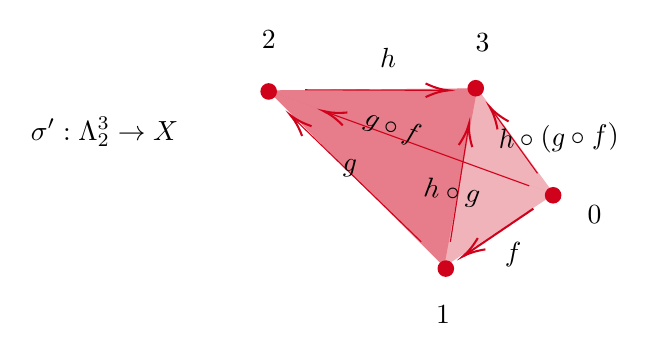
\begin{tikzpicture}[x=0.75pt,y=0.75pt,yscale=-1,xscale=1]
%uncomment if require: \path (0,300); %set diagram left start at 0, and has height of 300
%Shape: Boxed Line [id:dp712419722419394] 
\draw [draw opacity=0][fill={rgb, 255:red, 208; green, 2; blue, 27 }  ,fill opacity=0.3 ]   (277.11,135.11) -- (378.11,134.11) -- (415.11,185.11) -- cycle ;
%Shape: Boxed Line [id:dp06884731912188236] 
\draw [draw opacity=0][fill={rgb, 255:red, 208; green, 2; blue, 27 }  ,fill opacity=0.3 ]   (277.11,135.11) -- (362.11,220.11) -- (415.11,185.11) -- cycle ;
%Shape: Free Drawing [id:dp08767868053848638] 
\draw  [color={rgb, 255:red, 208; green, 2; blue, 27 }  ,draw opacity=1 ][line width=6] [line join = round][line cap = round] (277.58,135.63) .. controls (277.58,135.63) and (277.58,135.63) .. (277.58,135.63) ;
%Shape: Free Drawing [id:dp6329653420526828] 
\draw  [color={rgb, 255:red, 208; green, 2; blue, 27 }  ,draw opacity=1 ][line width=6] [line join = round][line cap = round] (362.92,220.97) .. controls (362.92,220.97) and (362.92,220.97) .. (362.92,220.97) ;
%Shape: Free Drawing [id:dp6342498607996421] 
\draw  [color={rgb, 255:red, 208; green, 2; blue, 27 }  ,draw opacity=1 ][line width=6] [line join = round][line cap = round] (414.62,185.65) .. controls (414.62,185.65) and (414.62,185.65) .. (414.62,185.65) ;
%Straight Lines [id:da526633051382492] 
\draw [color={rgb, 255:red, 208; green, 2; blue, 27 }  ,draw opacity=1 ]   (351.11,208.11) -- (289.55,148.5) ;
\draw [shift={(288.11,147.11)}, rotate = 44.08] [color={rgb, 255:red, 208; green, 2; blue, 27 }  ,draw opacity=1 ][line width=0.75]    (10.93,-3.29) .. controls (6.95,-1.4) and (3.31,-0.3) .. (0,0) .. controls (3.31,0.3) and (6.95,1.4) .. (10.93,3.29)   ;
%Shape: Free Drawing [id:dp44772844349269714] 
\draw  [color={rgb, 255:red, 208; green, 2; blue, 27 }  ,draw opacity=1 ][line width=6] [line join = round][line cap = round] (377.34,134.07) .. controls (377.34,134.07) and (377.34,134.07) .. (377.34,134.07) ;
%Straight Lines [id:da9429587691776815] 
\draw [color={rgb, 255:red, 208; green, 2; blue, 27 }  ,draw opacity=1 ][line width=0.75]    (405.11,192.11) -- (372.77,213.99) ;
\draw [shift={(371.11,215.11)}, rotate = 325.92] [color={rgb, 255:red, 208; green, 2; blue, 27 }  ,draw opacity=1 ][line width=0.75]    (10.93,-3.29) .. controls (6.95,-1.4) and (3.31,-0.3) .. (0,0) .. controls (3.31,0.3) and (6.95,1.4) .. (10.93,3.29)   ;
%Straight Lines [id:da7210386732599512] 
\draw [color={rgb, 255:red, 208; green, 2; blue, 27 }  ,draw opacity=1 ]   (295.1,134.83) -- (362.11,135.1) ;
\draw [shift={(364.11,135.11)}, rotate = 180.23] [color={rgb, 255:red, 208; green, 2; blue, 27 }  ,draw opacity=1 ][line width=0.75]    (10.93,-3.29) .. controls (6.95,-1.4) and (3.31,-0.3) .. (0,0) .. controls (3.31,0.3) and (6.95,1.4) .. (10.93,3.29)   ;
%Straight Lines [id:da9610602919544413] 
\draw [color={rgb, 255:red, 208; green, 2; blue, 27 }  ,draw opacity=1 ]   (365.11,208.11) -- (373.8,153.09) ;
\draw [shift={(374.11,151.11)}, rotate = 98.97] [color={rgb, 255:red, 208; green, 2; blue, 27 }  ,draw opacity=1 ][line width=0.75]    (10.93,-3.29) .. controls (6.95,-1.4) and (3.31,-0.3) .. (0,0) .. controls (3.31,0.3) and (6.95,1.4) .. (10.93,3.29)   ;
%Straight Lines [id:da8120815388496025] 
\draw [color={rgb, 255:red, 208; green, 2; blue, 27 }  ,draw opacity=1 ]   (403.11,181.11) -- (305.99,145.79) ;
\draw [shift={(304.11,145.11)}, rotate = 19.98] [color={rgb, 255:red, 208; green, 2; blue, 27 }  ,draw opacity=1 ][line width=0.75]    (10.93,-3.29) .. controls (6.95,-1.4) and (3.31,-0.3) .. (0,0) .. controls (3.31,0.3) and (6.95,1.4) .. (10.93,3.29)   ;
%Straight Lines [id:da274468734769862] 
\draw [color={rgb, 255:red, 208; green, 2; blue, 27 }  ,draw opacity=1 ]   (407.11,175.11) -- (385.28,144.74) ;
\draw [shift={(384.11,143.11)}, rotate = 54.29] [color={rgb, 255:red, 208; green, 2; blue, 27 }  ,draw opacity=1 ][line width=0.75]    (10.93,-3.29) .. controls (6.95,-1.4) and (3.31,-0.3) .. (0,0) .. controls (3.31,0.3) and (6.95,1.4) .. (10.93,3.29)   ;
%Shape: Boxed Line [id:dp5693420491484811] 
\draw [draw opacity=0][fill={rgb, 255:red, 208; green, 2; blue, 27 }  ,fill opacity=0.3 ]   (277.11,135.11) -- (378.11,134.11) -- (362.11,220.11) -- cycle ;
% Text Node
\draw (161.73,146.92) node [anchor=north west][inner sep=0.75pt]    {$\sigma ':\Lambda _{2}^{3}\rightarrow X$};
% Text Node
\draw (357,237.4) node [anchor=north west][inner sep=0.75pt]    {$1$};
% Text Node
\draw (273.02,105.17) node [anchor=north west][inner sep=0.75pt]    {$2$};
% Text Node
\draw (430,189.4) node [anchor=north west][inner sep=0.75pt]    {$0$};
% Text Node
\draw (376,106.4) node [anchor=north west][inner sep=0.75pt]    {$3$};
% Text Node
\draw (390.11,207.01) node [anchor=north west][inner sep=0.75pt]    {$f$};
% Text Node
\draw (312,167.4) node [anchor=north west][inner sep=0.75pt]    {$g$};
% Text Node
\draw (325.43,141.38) node [anchor=north west][inner sep=0.75pt]  [rotate=-19.28]  {$g\circ f$};
% Text Node
\draw (330,113.4) node [anchor=north west][inner sep=0.75pt]    {$h$};
% Text Node
\draw (351.95,175.66) node [anchor=north west][inner sep=0.75pt]  [rotate=-6.42]  {$h\circ g$};
% Text Node
\draw (386.69,151.9) node [anchor=north west][inner sep=0.75pt]  [rotate=-357.41]  {$h\circ ( g\circ f)$};
        \end{tikzpicture}\]
        它有唯一的延拓
        \[\begin{tikzcd}
	& 1 \\
	0 && 3
	\arrow["{h\circ g}", from=1-2, to=2-3]
	\arrow["f", from=2-1, to=1-2]
	\arrow["{(h\circ g)\circ f}"', from=2-1, to=2-3]
        \end{tikzcd}\]
        依照如上构造,上述$2$-单形确定了$f$与$h\circ g$的合成,即$(h\circ g) \circ f= h\circ (g\circ f)$(即图中$0 \to 3$的两种合成是一致的).\\
        
        综上, $\mathcal{C}$是范畴有典范态射$X\to \nerve\mathcal{C}$,方式为给定$\Delta^n \to X$沿着各个$\Delta^1\xrightarrow{\{j,j+1\}}\Delta^n$拉回以得到态射链.由构造显然有$X_n \to \nerve \mathcal{C}_n$在$n = 0,1$时是双射.在$n \geq 2$时,取$0<i<n$并考虑图表
        \[\begin{tikzcd}
	{\Hom(\Delta^n,X)} & {\Hom(\Delta^n,\nerve \mathcal{C})} \\
	{\Hom(\Lambda_i^n,X)} & {\Hom(\Lambda_i^n,\nerve\mathcal{C})}
	\arrow[from=1-1, to=1-2]
	\arrow["{\text{双射}}"', from=1-1, to=2-1]
	\arrow["{\text{双射}}", from=1-2, to=2-2]
	\arrow[from=2-1, to=2-2]
    \end{tikzcd},\]
    由命题\ref{Pro:边界与尖角图表}可知$\Lambda_i^n$可表为一族$\Delta^{n-1}$和$\Delta^{n-2}$的$\Coker$.由$n=0,1$进行递归即可得知第二行为双射,因此图表交换.
    \item[2. $\Rightarrow$ 3.]通过对$n$进行归纳来证明,当$n = 2$时, $I^2 : 0 \to 1 \to 2$即为内尖角$\Lambda_1^2$根据假设自然满足唯一填充性质.接下来假设对于$k<n$的情况均具有填充性质,现在我们需要将脊$I^n\to X$延拓为$\Delta^n \to X$.观察到$I^n \cap \Delta^{[n]\setminus \{n\}}$即为$I^{n-1}$,同理$I^n \cap \Delta^{[n]\setminus\{0\}}$也是脊.因此根据归纳假设,对于$j = 0,n$存在唯一延拓$\Delta^{[n]\setminus\{j\}}\to X$.考虑两个面的交,即为$\Delta^{[n]\setminus\{0,n\}}$,再交上脊即可得到一个更小的脊,根据假设,两个延拓在相交处是相等的.因此得到映射
    \[
    I^n \cup \Delta^{[n]\setminus\{0\}}\cup\Delta^{[n]\setminus\{n\}} = \Delta^{[n]\setminus\{0\}}\cup\Delta^{[n]\setminus\{n\}} \to X
    \]
    且并起来就是$\Delta^n$.断言存在唯一延拓
    \[\Delta^{[n]\setminus\{0\}}\cup\Delta^{[n]\setminus\{n\}}\cup\Delta^{[n]\setminus\{1\}}\]
    为证明断言,先说明$\Delta^{[n]\setminus\{0\}}\cup\Delta^{[n]\setminus\{n\}}$包含$\Delta^{[n]\setminus\{1\}}$的脊:这是因为$2\leq \leq n-1$与$i \to i+1$均在$\Delta^{[n]\setminus\{0\}}$中,而$0 \to 2$在$\Delta^{[n]\setminus\{n\}}$中($n\geq 3$).因此,由脊可以扩充出唯一的$\Delta^{[n]\setminus\{1\}}\to X$,还需要证明它们在相交处
    \[
    (\Delta^{[n]\setminus\{n\}}\cup \Delta^{[n]\setminus\{0\}})\cap \Delta^{[n]\setminus\{1\}} = \Delta^{[n]\setminus\{1,n\}}\cup \Delta^{[n]\setminus\{0,1\}}.
    \]
    是一致的.而在这些单形中,映射实际上都被在它们的脊所决定,因此得知断言成立.进行归纳即可得到存在唯一的映射$\Lambda_{n-1}^n \to X$,而根据条件2.可以得知这个映射唯一延拓到$\Delta^n$上.
    \item[3. $\Rightarrow$ 2.]考虑单纯集间的映射$\beta : \Lambda_i^n \to X$,需要说明它能够唯一地扩张到$\Delta^n$上.在$n = 2$时, $I^2 : 0 \to 1 \to 2$即为内尖角$\Lambda_1^2$根据假设自然满足唯一填充性质.考虑$n \geq 3$时,有嵌入$I^n \hookrightarrow \Lambda_i^n$根据3.可知存在唯一延拓$\alpha :\Delta^n \to X$.再将这个延拓限制到$\Lambda_i^n$,我们只需要证明$\alpha \mid_{\Lambda_i^n} = \beta$.由于$\Lambda_i^n = \bigcup_{j \neq i}\Delta^{[n]\setminus\{j\}}$,因此可以将问题化约到$\Lambda_i^n$的每个面上进行证明.不难看出
    \[
    \alpha\mid_{\Delta^{[n]\setminus\{0\}}} = \beta\mid_{\Delta^{[n]\setminus\{0\}}}
    \]
    由于这个单纯集的脊是脊$I^n$的子集,并且根据定义有$\alpha \mid_{I^n} = \beta\mid_{I^n}$.因此可以推广为
    \[
    \alpha\mid_{\Delta^{[n]\setminus\{n\}}} = \beta\mid_{\Delta^{[n]\setminus\{n\}}}
    \]
    还需要证明的是
    \[
    \alpha\mid_{\Delta^{[n]\setminus\{j\}}} = \beta\mid_{\Delta^{[n]\setminus\{j\}}}
    \]
    根据假设知$j \neq 0,n$. 首先证明$\alpha\mid_{\Delta^{[n]\setminus\{j-1,j+1\}}} = \beta\mid_{\Delta^{[n]\setminus\{j-1,j+1\}}}$,根据2. $\Rightarrow$ 3.的讨论已然得知这些边要么在$\Delta^{[n]\setminus \{0\}}$中要么在$\Delta^{[n]\setminus \{n\}}$中.因此证明完成.
    \end{enumerate}
\end{proof}
\begin{remark}\label{Rk:外尖角可填充为群胚}
    不难发现,若要求条件2.的适用范围扩大到外尖角上,则$\mathcal{C}$是群胚.只需要取$\Lambda_0^2$, $K$为单纯集的脉,给定映射$\Lambda_0^2 \to K$其对应于
    \[\begin{tikzcd}
	& {C_1} \\
	{C_0} && {C_2}
	\arrow[from=1-2, to=2-3]
	\arrow[dashed, from=2-1, to=1-2]
	\arrow[from=2-1, to=2-3]
    \end{tikzcd}\]
    取$C_0 \to C_2 = \identity$, $C_1 \to C_2 = f$则尖角填充性质说明$f$可逆.
\end{remark}

记$\cate{Cat}$是所有小范畴构成的范畴,态射取为函子.任意函子$F : \mathcal{C} \to \mathcal{C}'$都诱导$\cate{sSet}$中的态射$\nerve F : \nerve \mathcal{C} \to \nerve \mathcal{C}' , (f_1,\cdots,f_n) \to (Ff_1,\cdots,Ff_n)$,由此定义出脉函子$\nerve : \cate{Cat} \to \cate{sSet}$.
\begin{corollary}
    脉函子是全忠实的.
\end{corollary}
\begin{proof}
    根据命题\ref{Pro:脉的刻画}可知$\nerve \mathcal{C} \to \nerve \mathcal{C}'$自然诱导$\mathcal{C}\to \mathcal{C}'$.不难发现与$\nerve$诱导的态射互逆,因此为态射集间的双射,即全忠实.
\end{proof}
\section{Dold-Kan 对应}\label{Dold-Kan 对应}
\begin{wenxintishi}
    本文讲述单纯集上的 Dold-Kan 对应,而 $\infty$-范畴上的版本将在后文讲述.
\end{wenxintishi}
\subsection{Dold-Kan}
令$\mathcal{A}$为加性小范畴,从$\mathcal{A}$出发可以定义单形对象范畴$\mathsf{s}\mathcal{A}$以及链复形范畴$\Chain(\mathcal{A})$.本节主要考虑的是其子范畴$\Chain_{\geq 0}(\mathcal{A})$(见约定\ref{约定:链复形范畴})本节的目的是明确这两个范畴之间的关系,或者精确一点的说,我们将定义三个函子
\[\begin{tikzcd}
	{\Chain_{\geq 0}(\mathcal{A})} & {\mathsf{s}\mathcal{A}}
	\arrow["\DK"{description}, from=1-1, to=1-2]
	\arrow["\chain_*"{description}, curve={height=18pt}, from=1-2, to=1-1]
	\arrow["\normal_*"{description}, curve={height=-18pt}, from=1-2, to=1-1]
\end{tikzcd}\]
接下来我们进行一番婚丧嫁娶将这三个函子的定义叙述
\begin{definition}[非正规化链复形]
    对于$\mathcal{A}$中的半单纯形对象$X$和每个$n\in \Z_{\geq 1}$,定义
    \[
    \partial_n := \sum_{i =0}^n (-1)^i d_i :X_n \to X_{n-1};
    \]
    这使得$(X_n)_{n\geq 0}$连同$(\partial_n)_n$构成$\Chain(\mathcal{A})$中的对象,称为$X$所给出的非正规化链复形或 Moore 链复形,记为 $\chain_*(X)$;因此$\chain_n(X) = X_n$.
\end{definition}
在代数拓扑中我们已经知道$n >1$时$\partial_{n-1} \partial_n = 0$;当然我们可以再重新提一遍,由注记\ref{注记:面态射与退化态射}可知$i<j \Rightarrow d_id_j = d_{j-1}d_i$这也说明
\begin{align*}
    \partial_{n-1}\partial_n = \sum_{i=0}^{n-1}\sum_{j=0}^n (-1)^{i+j}&d_id_j\\
    &= \sum_{0\leq i<j \leq n}(-1)^{i+j}d_{j-1}d_i + \sum_{n-1 \geq i \geq j \geq 0}(-1)^{i+j}d_id_j = 0.
\end{align*}
此构造对于$X$是典范的,这给出函子$\chain_*$.
\begin{definition}[Dold-Kan 构造]
    取定$\Chain_{\geq 0}(\mathcal{A})$中的对象$(A_n,\partial_n)_{n\geq 0}$.依照如下方式定义$\mathsf{s}\mathcal{A}$中对象$\DK(A)$.
    \[
    \DK_n(A) := \bigoplus_{t: [n] \twoheadrightarrow [k]}A_k.
    \]
    对于$\Delta$的任意态射$f: [m] \to [n]$,对应的$f^*: \DK_n (A) \to \DK_m (A)$相对于上述直和分解表为以下矩阵
    \[
    (\Phi_{u,t}:A_k \to A_l)_{\substack{u:[m]\twoheadrightarrow[l]\\t:[n]\twoheadrightarrow[k]}},
    \]
    按照以下方式确定:给定$t :[n] \twoheadrightarrow [k]$,做$tf$的满-单分解
    \begin{equation}\label{公式:满单分解}
    \tag{满-单分解}
        \begin{tikzcd}
	& {[n]} \\
	{[m]} && {[k]} \\
	& {[l]}
	\arrow["t", two heads, from=1-2, to=2-3]
	\arrow["f", from=2-1, to=1-2]
	\arrow["u"', two heads, from=2-1, to=3-2]
	\arrow["v"', hook, from=3-2, to=2-3]
        \end{tikzcd}
    \end{equation}
    \begin{itemize}
        \item 若$l = k$,命$\Phi_{u,t} = \identity$;
        \item 若$l = k-1$,而$v = \delta^0$(遗漏$0$的保序单射),命$\Phi_{u,t} = \partial_k : A_k \to A_{k-1}$;
        \item 其余情形命$\Phi_{u,t}=0$.
    \end{itemize}
    注意到当$f$与$t$给定时,至多存在唯一的$u$使得$\Phi_{u,t} \neq 0$.称其为 Dold-Kan 构造.
\end{definition}
可以验证$\DK A\in \Obj (\mathsf{s}\mathcal{A})$,核心是$(\DK \mathcal{A})_n$的直和项$A_n$和它们在保序单态射下的行为,其它低次直和项$A_k$皆来自满态射$[n]\twoheadrightarrow [k]$诱导的退化,一般情况下$f^*$的定义不过是体现此思路.\\
以上构造是典范的,给出函子$\DK : \Chain_{\geq 0}(\mathcal{A}) \to \mathsf{s} \mathcal{A}$.
\begin{definition}[正规化链复形]
    设$\mathcal{A}$是 Abel 范畴.对$\mathcal{A}$中的半单纯形对象$X$和所有$n\in \Z_{\geq 0}$和$0 \leq k \leq n$定义
    \begin{align*}
        \normal_n(X)&:= \bigcap_{i=1}^n \ker[d_i : X_n \to X_{n-1}], &n \geq 1,\\
        \normal_0(X)&:= X_0.&
    \end{align*}
    连同$X_n \xrightarrow{d_0}X_{n-1}$所诱导的态射族$\normal_n (X) \to \normal_{n-1}(X)$.合理地记为$\partial_n$,它们构成$\Chain_{\geq 0}(\mathcal{A})$中的对象$\normal_*(X)$,称为$X$的正规化链复形.
\end{definition}
\begin{proposition}\label{命题:自然嵌入u_n}
    对如上定义的$X$和每个$n \geq 0$,记$u_n :\normal_n(X) \hookrightarrow X_n$为自然嵌入,则$(u_n)_{n \geq 0}$构成$\Chain_{\geq 0}(\mathcal{A})$中的单态射$u : \normal_*(X) \to \chain_*(X)$,它对$X$满足函子性.
\end{proposition}
\begin{proof}
    直接来自于$\normal_*$和$\chain_*$的定义.
\end{proof}
而后对于 Dold-Kan 定理进行一些必要的铺垫.
\begin{lemma}\label{引理:NDK(A)}
    设$\mathcal{A}$是 Abel 范畴,则对所有的$A\in \Obj(\Chain_{\geq 0}(\mathcal{A})$和$n \geq 0$有$\normal_n \DK(A) = A_n$.这给出函子的同构$\eta : \identity_{\Chain_{\geq 0}(\mathcal{A})} \rightiso \normal_* \DK$.
\end{lemma}
\begin{proof}
    给定$t:[n] \twoheadrightarrow [k]$,注意到当$k<n$时,总可以取$1\leq i \leq n$使得$t^{-1}(t(i))$至少有两个元素,从而$t\delta^i$满,使下图交换
    \[\begin{tikzcd}
	& {[n]} \\
	{[n-1]} && {[k]} \\
	& {[k]}
	\arrow["t", two heads, from=1-2, to=2-3]
	\arrow["{\delta^i}", from=2-1, to=1-2]
	\arrow["{t\delta^i}"', two heads, from=2-1, to=3-2]
	\arrow["\identity"', from=3-2, to=2-3]
    \end{tikzcd}\]
    由此可知$\normal_n \DK(\mathcal{A})$包含于$\identity:[n]\to [n]$对应的直和项$A_n$.然而易证该定义进一步蕴涵$\normal_n \DK(A) = A_n$.而且$\normal_{n+1}\DK(A) \to \normal_n\DK(A)$正是$\partial_{n+1}:A_{n+1}\to A_n$.
\end{proof}
\begin{lemma}\label{引理:DK与N_*伴随}
    设$\mathcal{A}$为 Abel 范畴,先前定义的函子给出伴随对
    \[
    \DK : \Chain_{\geq 0}(\mathcal{A}) \leftrightarrows \mathsf{s} \mathcal{A} : \normal_*
    \]
    \begin{itemize}
        \item 对应的单位态射为引理\ref{引理:NDK(A)}中的$\eta$;
        \item 余单位态射$\varepsilon : \DK \normal_* \to \identity_{\mathsf{s}\mathcal{A}}$描述如下:给定$t : [n] \twoheadrightarrow [k]$,在$\DK \normal_n(X)$中相应的直和项$\normal_k(X)$上,$\varepsilon_{X,n}$是$\normal_k(X) \subset X_k \xrightarrow{t^*}X_n$.
    \end{itemize}
\end{lemma}
\begin{proof}
    给定$A\in \Obj(\Chain_{\geq 0}(\mathcal{A}))$和$X\in \Obj(\mathsf{s}\mathcal{A})$,首要目标是证明
    \[
    \Hom_{\mathsf{s}\mathcal{A}}(\DK(A),X) \xrightarrow{\normal} \Hom_{\Chain_{\geq 0}(\mathcal{A})}(\normal_*\DK(A),\normal_*(X)) \xrightarrow{\eta_A^*}\Hom_{\Chain_{\geq 0}(\mathcal{A})}(A,\normal_*(X))
    \]
    合成为双射.其逆的具体定义如下.给定$\phi = (\phi_n)_{n \geq 0}: A \to \normal_*(X)$,定义态射
    \[
    \Phi_m: (\DK A)_n = \bigoplus_{t: [n] \twoheadrightarrow [k]}A_k \to X_n
    \]
    使得它在对应$t: [n] \twoheadrightarrow [k]$的直和项上是
    \[
    A_k \xrightarrow{\phi_k}\normal_k(X) \subset X_k \xrightarrow{t^*}X_n
    \]
    的合成.对于如上的$t$和任意$f : [m] \to [n]$可做$f$的满-单分解(\ref{公式:满单分解}),并考虑$\mathcal{A}$中的图表
    \[\begin{tikzcd}
	{A_k} & {\normal_k(X)} & {X_k} & {X_n} \\
	{A_l} & {\normal_l(X)} & {X_l} & {X_m}
	\arrow["{\phi_k}", from=1-1, to=1-2]
	\arrow["{\Phi_{u,t}}"', from=1-1, to=2-1]
	\arrow[hook, from=1-2, to=1-3]
	\arrow["{v^*\mid_{\normal_k(X)}}", from=1-2, to=2-2]
	\arrow["{t^*}", from=1-3, to=1-4]
	\arrow["{v^*}", from=1-3, to=2-3]
	\arrow["{f^*}", from=1-4, to=2-4]
	\arrow["{\phi_l}"', from=2-1, to=2-2]
	\arrow[hook, from=2-2, to=2-3]
	\arrow["{u^*}"', from=2-3, to=2-4]
    \end{tikzcd}\]
    左侧方块由$\normal_*(X)$定义可知交换性,中间方块的交换性是显然的,右侧由$tf = vu$所确定.取$\phi \mapsto \Phi$中取$\phi = \identity_{\normal_*(X)}$即可得到余单位态射.
\end{proof}
\begin{lemma}\label{引理:DK在 Ab 上为 伴随等价}
    取$\mathcal{A} = \cate{Ab}$,则$\DK$为等价;或者说$\DK : \Chain_{\geq 0}(\cate{Ab}) \leftrightarrows \cate{sAb}: \normal$为伴随等价.
\end{lemma}
\begin{proof}
    由\parencite[定理 2.6.12.]{李文威卷一}可知,只需要说明余单位态射$\varepsilon$是同构即可.给定$X\in \Obj(\mathsf{s}\mathcal{A})$,我们来验证$\varepsilon_{X,n}: \DK(\normal_*(X))_n \to X_n$对于每个$n \geq 0$即单又满.
    \begin{enumerate}
        \item[单性] 设$x = (x_t)_t \in \DK(\normal_*(X))_n$,其中$t$遍历保序满射$[n] \twoheadrightarrow [k]$.给定$t$,定义保序单射
        \begin{align*}
        s = s_t :[k] &\hookrightarrow [n]\\
         i &\mapsto \min t^{-1}(i)
        \end{align*}
        它满足$ts = \identity_{[k]}$.现在假定$x \neq 0$,记
        \[
        S := \{t : x_t \neq 0\}\neq \varnothing
        \]
        取最小的$k$使得存在属于$S$的$t : [m] \twoheadrightarrow [k]$,再取如此的$t$使得$\sum_{i=0}^k \min t^{-1}(i)$尽可能小,并构造$s$.现在证明$s^*(\varepsilon_{X,n}(x)) = x_t \in X_k$,以此说明$\varepsilon_{X,n}(x) \neq 0$.\\
        基于$\varepsilon_{X,n}$的具体描述,仅需对$t':[n] \twoheadrightarrow [k']$证明$s^*(t')^*(x_{t'}) \neq 0$蕴含$t = t'$即可.命$u := t' s: [k] \to [k']$.当$t' \notin S$时$x_{t'} =0$,故假设$t' \in S$满足$s^*(t')^*(x_{t'}) = u^*(x_{t'}) \neq 0$.\\
        由于$t$保序且为满射,因此$\min t^{-1}(0) =0$,对$t'$亦然,故$u(0) = 0$.又由$x_{t'}\in \normal_{k'} (X)$可推知仅当$\Image(u) \supset \{1,\cdots,k'\}$时才能有$u^*(x_{t'}) \neq 0$.故假设$u$为满, $k$的取法自然蕴含$k'= k$而$u = \identity$.\\
        从而得出$t'(\min t^{-1}(i)) = i$对于$i =  0,\cdots, k$成立,故$\min (t')^{-1}(i) \leq \min t^{-1}(i)$.回顾$t$的取法可知$\min (t')^{-1}(i) = \min t^{-1}(i)$,即$t = t'$.从而$\varepsilon_{X,n}$单.
        \item[满性]通过对$n$递归地证明$\varepsilon_{X,n}$满.兹断言对所有$0 \leq i \leq n$都有
        \[
        \Image(\varepsilon_{X,n})\supset X(i)_n := \bigcap_{i < j \leq n}\ker(d_j) \subset X_n
        \]
        当$i = 0$时 $X(i)_n = \normal_n(X)$,上式容易从$\varepsilon_{X,n}$的具体描述中导出,而我们的目标为$i = n$的情况.现设$n\geq i \geq 1$而$y\in X(i)_n$.关于$n-1$的递归假设和$\varepsilon_{X,n}$蕴含
        \[
        s_{i-1}d_i(y) \in s_{i-1}(\Image(\varepsilon_{X,n-1})) \subset \Image(\varepsilon_{X,n}).
        \]
        另一方面,由于$d_is_{i-1}d_i = d_i d_{i}s_{i} = d_i$以及$j >i$时,$d_j s_{i-1} d_i = s_{i-1} d_{j-1} d_i = s_{i-1} d_i d_j$.因此$y - s_{i-1}d_i (y) \in X(i-1)_n$,由关于$i-1$的递归假设可知其属于$\Image(\varepsilon_{X,n})$.综上$y\in \Image(\varepsilon_{X,n})$.明所欲证.
    \end{enumerate}
\end{proof}
回忆到在 Abel 范畴中我们曾定义幂等元$e\in \End(\mathcal{A})$为满足$e\circ e = e^2 = e$的态射,并且所有幂等元均有核的具有零对象的 $\dcate{Ab}$范畴称为 Karoubi 范畴,接下来介绍本节的核心定理.
\begin{theorem}[A. Dold, D. Kan]
    对于任意加性范畴$\mathcal{A}$,函子$\DK : \Chain_{\geq 0}(\mathcal{A}) \to \mathsf{s} \mathcal{A}$是全忠实的.
    \begin{enumerate}
        \item 若$\mathcal{A}$还是 Karoubi 范畴,则$\DK$为范畴等价.
        \item 若$\mathcal{A}$为 Abel 范畴,则 $\normal_*$ 为 $\DK$ 的拟逆函子$\DK : \Chain_{\geq 0}(\mathcal{A}) \leftrightarrows \mathsf{s} \mathcal{A} : \normal_*$为伴随等价,伴随对的单位和余单位态射由引理\ref{引理:DK与N_*伴随}给出.
    \end{enumerate}
\end{theorem}
\begin{proof}
    考虑函子
    \begin{align*}
    \tilde{h}_{\cal{A}}: \cal{A} &\to \tilde{\cal{A}}^{\land} := \cate{Ab}^{(\cal{A})^{\opposite}}\\
    Y &\mapsto \Hom_{\cal{A}}(-,Y)
    \end{align*}
    它与忘却函子的合成等于Yoneda嵌入$h_{\cal{A}} : \cal{A} \to \cal{A}^{\land}$.函子$\tilde{h}_{\cal{A}}$是全忠实的,这点不过是 $\cate{Ab}$-版本的Yoneda 引理,可以从原版推导:对于任意$Y_1 ,Y_2 \in \Obj(\cal{A})$,合成映射
    \[
    \Hom_{\cal{A}}(Y_1,Y_2) \to \Hom_{\tilde\cal{A}^{\land}}\left(\tilde{h}_{\cal{A}}(Y_1),\tilde{h}_{\cal{A}}(Y_2)\right)\to \Hom_{\cal{A}^{\land}}\left(h_{\cal{A}}(Y_1),h_{\cal{A}}(Y_2)\right)
    \]
    不难发现复合即为双射,而右侧箭头显然单,因此为双射.接下来回归正题.由于$\tilde{A}^{\land}= \cate{Ab}^{(\cal{A})^{\opposite}}$,因此由 $\cate{Ab}$为 Abel 范畴可知$\cate{Ab}^{(\cal{A})^{\opposite}}$为 Abel 范畴.以相同的符号标记$\tilde{h}_{\cal{A}}$在链复形和单纯形对象上诱导的函子,考虑图表
    \[\begin{tikzcd}
	{\Chain_{\geq 0}(\cal{A})} & {\mathsf{s}\cal{A}} \\
	{\Chain_{\geq 0}(\tilde{\cal{A}}^{\land})} & {\mathsf{s}\tilde{\cal{A}}^{\land}}
	\arrow["\DK", from=1-1, to=1-2]
	\arrow["{\tilde{h}_{\cal{A}}}"', from=1-1, to=2-1]
	\arrow["{\tilde{h}_{\cal{A}}}", from=1-2, to=2-2]
	\arrow["\DK"', from=2-1, to=2-2]
    \end{tikzcd}\]
    此图精确到典范同构是交换的.上一段的观察说明两个垂直箭头全忠实,而逐对象地使用关于$\cate{Ab}$的引理\ref{引理:DK在 Ab 上为 伴随等价},可见第二行也为范畴等价,于是第一行$\DK$为全忠实.\\

    对于任意函子$F: \cal{C} \to \cal{C}'$,我们称$X'\in \Obj(\cal{C}')$属于$F$的本质像,如果存在$X\in \Obj(\cal{C})$使得$X'\simeq FX$.搭配引理\ref{引理:DK在 Ab 上为 伴随等价}对于$\Chain_{\geq 0} \to \cate{sAb}$的拟逆的描述,便可以得到以下结论:$X\in \Obj(\cate{s}\cal{A})$属于$\DK$的本质像当且仅当$\normal_n\tilde{h}_{\cal{A}}(X)$对每个$n \geq 0$皆属于$\tilde{h}_{\cal{A}}: \cal{A} \to \tilde{\cal{A}}^{\land}$的本质像.\\
    注意到$\tilde{h}_{\cal{A}}: \cal{A} \to \tilde{\cal{A}}^{\land}$保持有限直和.当$\cal{A}$为 Karoubi 范畴时, $\cal{A} \to \tilde{\cal{A}}^{\land}$的本质像因而对萃取直和项保持封闭;既然$\normal_n\tilde{h}_{\cal{A}}(X)$是$\DK\normal_n\tilde{h}_{\cal{A}}(X)\simeq h_{\cal{A}}(X)_n$的直和项,此时$\DK$全忠实本质满,从而为等价.\\
    最后使用\parencite[定理 2.6.12]{李文威卷一}的伴随等价定理,其确保$\DK$的拟逆总是能扩充为右伴随.当$\cal{A}$为 Abel 范畴时,引理\ref{引理:DK与N_*伴随}已然说明$\normal$为$\DK$的右伴随,从而为拟逆.
\end{proof}
\begin{notation}
    基于此,当$\cal{A}$为 Karoubi 范畴时,可以选定$\DK : \Chain_{\geq 0}(\cal{A}) \to \sf{s}\cal{A}$的拟逆函子,记为$\normal_*$.
\end{notation}
虽然$\normal_*(X)$的初始定义为$\chain(X)$的子对象,但是将其理解为商是更为方便的.以下来说明这一点.\\
考虑 Karoubi 范畴$\cal{A}$以及$X\in \Obj(\sf{s}\cal{A})$对所有$n \geq 0$定义$\cal{A}$中态射$\Psi_n$,其刻画是使得下图对所有$0 \leq j <n$交换
\[\begin{tikzcd}
	{\bigoplus_{0\leq i <n}X_{n-1}} & {X_n} \\
	{X_j}
	\arrow["{\Psi_n}", from=1-1, to=1-2]
	\arrow["{\text{直和项}}", hook, from=2-1, to=1-1]
	\arrow["{s_j}"', from=2-1, to=1-2]
\end{tikzcd}\]
因此考虑$\Coker(\Psi_n)$相当于从$X$中抹去退化部分,至少在$\cal{A}$为 Abel 范畴时可以这么想;次一则结果将说明$\Coker(\Psi_n)$不仅存在还可以通过命题\ref{命题:自然嵌入u_n}中描绘的自然嵌入$u : \normal_*(X) \to \chain_*(X)$来等同于$\normal_n(X)$,这提供了看待$\normal_*(X)$的另一视角.
\begin{proposition}
    上述情境中, $\Coker(\Psi_n)$存在并且典范同构于$\normal_n(X)$,考虑相应的合成$v_n : X_n \twoheadrightarrow \Coker(\Psi_n) \rightiso \normal_n(X)$,则$(v_n)_n$给出态射$v : \chain_*(X) \to \normal_*(X)$它对于$X$具有函子性,并且对于自然嵌入$u : \normal_*(X) \to \chain_*(X)$有$vu = \identity_{\normal_*(X)}$.
\end{proposition}
\subsection{同调计算}
\section{Eilenberg-Zilber定理}\label{Eilenberg-Zilber定理}
\section{统联,锥,映射锥}
本节讲述单纯集的锥这一概念,这一概念实际上牵扯到后文中关于态射空间的很多构造,也与同调代数中映射锥的概念是相关的.\\
记$\cate{FinLin}_{+}$为从有限全序集范畴$\cate{FinLin}$去掉空集所构成的全子范畴,不难发现$\Delta$为其一副骨架,单纯形集可以理解为$\cate{FinLin}_+^{\opposite} \to \cate{Set}$.
%\begin{convention}
%    设$J\in \cate{FinLin}_+$为对象.任意子集$I \subset J$自动为有限全序集;若还有
%    \[
%    \forall  (i,j) \in I \times J, j\leq i \Rightarrow j\in I
%    \]
%    则称$I$为$J$的一个前段,记为$I \sqsubset J$.
%\end{convention}
我们先给出范畴中统联的定义
\begin{definition}
    对于范畴$\mathcal{C}$, $\mathcal{C}'$,定义其统联$\mathcal{C} \star \mathcal{C}'$如下:
    \begin{itemize}
        \item $\Obj(\mathcal{C} \star \mathcal{C}') := \Obj(\mathcal{C}) \sqcup \Obj(\mathcal{C}')$.
        \item $\Hom$集构造如下
        \[
        \Hom_{\mathcal{C}\star \mathcal{C}'} := \left\{
        \begin{array}{ccc}
             \Hom_{\mathcal{C}}(X,Y),&X,Y\in \Obj(\mathcal{C})  \\
             \Hom_{\mathcal{C}'}(X,Y),& X,Y\in \Obj(\mathcal{C}')  \\
             \text{单点集}\{*\}, & X\in \Obj(\mathcal{C}),Y\in \Obj(\mathcal{C}'),\\
             \varnothing, & X\in \Obj(\mathcal{C}'),Y\in \Obj(\mathcal{C}),
        \end{array}{ccc}
        \right.
        \]
    \end{itemize}
\end{definition}
$\mathcal{C}\star \mathcal{C}'$以自明的方式构成范畴,不难发现统联不是对称的.为定义出单纯集上的统联,我们需要引入分划这一概念
\begin{definition}[分划]
    给定全序集$J$,定义$\cate{Cut}(J)$为
\end{definition}
\section{本讲习题}